\documentclass[12pt]{article}

\usepackage{amsmath}
\usepackage{amsfonts}
\usepackage{amssymb}
\usepackage{amsthm}
\usepackage{stmaryrd}
\usepackage{centernot}
\usepackage{tikz}
\usepackage{hyperref}
\usepackage[capitalise,poorman,nameinlink]{cleveref}


\newcommand{\typeeq}{\simeq} % Type equal
\newcommand{\ntypeeq}{\not\typeeq} % Not type equal

\newcommand{\ccharb}{:\empt:} % character for empty type in commands TODO DELETE
\newcommand{\ccharf}{:\mathtt{F}:} % Character for file type in commands TODO DELETE
\newcommand{\cchard}{:\mathtt{D}:} % Character for dir type in commands TODO DELETE

\newcommand{\vald}{\mathtt{D}} % Directory value
\newcommand{\valdi}{\mathtt{D}_1}
\newcommand{\valdii}{\mathtt{D}_2}
\newcommand{\valf}{\mathtt{F}_i} % File value
\newcommand{\valff}{\mathtt{F}_j} % File value
\newcommand{\fil}{\mathtt{F}_0} % Selected file value for representative objects
\newcommand{\empt}{\ominus} % Empty value
\newcommand{\valv}{v} % Any value
\newcommand{\valvy}{:v_Y:} % TODO DELETE
\newcommand{\valvw}{:v_W:} % TODO DELETE

\newcommand{\setfs}{\mathbb{F}_\setn} % Set of filesystems
\newcommand{\setv}{\mathbb{V}} % Set of values
\newcommand{\setn}{\mathbb{N}} % Set of nodes / paths
\newcommand{\sets}{\mathbb{S}} % Set of sequences
\newcommand{\setsmin}{\sets_{\mathrm{min}}} % Set of minimal sequences
\newcommand{\setssmp}{\sets_{\mathrm{simple}}} % Set of simple sequences
\newcommand{\setvx}[1]{\setv_{#1}} % Set of values with custom index
\newcommand{\setd}{\setvx{\vald}} % Set of directory values
\newcommand{\setb}{\setvx{\empt}} % Set of empty values TODO DELETE

\newcommand{\parent}{\text{\normalfont\scshape{parent}}} % parent function symbol
\newcommand{\parentf}[1]{\parent(#1)} % parent function
\newcommand{\fsbroken}{\bot} % value when command is not defined / broken FS value
\newcommand{\FS}{\Phi} % a filesystem
\newcommand{\GS}{\Theta} % another filesystem
\newcommand{\aFS}{\,\FS} % a filesystem preceded by something applied to it
\newcommand{\aGS}{\,\GS} % a filesystem preceded by something applied to it
\newcommand{\nn}{n'} % parent node
\newcommand{\T}{\tau} % type-equivalent class mapping

\newcommand{\cbrk}{c_\varnothing} % 'break' / empty command

\newcommand{\caa}[2]{\langle{[#1],[#2]}\rangle} % Command template
\newcommand{\caaa}[3]{\langle{[#1],#2,#3}\rangle}
\newcommand{\caaaa}[3]{\langle{[#1],#2,#3}\rangle}
\newcommand{\cTaaa}[3]{\langle{[#1],{#2}\T,#3}\rangle} % Representative of command

\newcommand{\cbb}{\caa{\empt}{\empt}}
\newcommand{\cbba}[1]{\caaa{\empt}{\empt}{#1}}
\newcommand{\cbf}{\caa{\empt}{\valf}}
\newcommand{\cbfaa}[1]{\caaa{\empt}{\valf}{#1}}
\newcommand{\cbd}{\caa{\empt}{\vald}}
\newcommand{\cbdaa}[1]{\caaa{\empt}{\vald}{#1}}
\newcommand{\cfb}{\caa{\valf}{\empt}}
\newcommand{\cfba}[1]{\caaa{\valf}{\empt}{#1}}
\newcommand{\cff}{\caa{\valf}{\valf}}
\newcommand{\cfd}{\caa{\valf}{\vald}}
\newcommand{\cfdaa}[1]{\caaa{\valf}{\vald}{#1}}
\newcommand{\cdb}{\caa{\vald}{\empt}}
\newcommand{\cdba}[1]{\caaa{\vald}{\empt}{#1}}
\newcommand{\cdf}{\caa{\vald}{\valf}}
\newcommand{\cdfaa}[1]{\caaa{\vald}{\valf}{#1}}
\newcommand{\cdd}{\caa{\vald}{\vald}}
\newcommand{\cdda}[1]{\caaa{\vald}{\vald}{#1}}

\newcommand{\cxy}{\caa{x}{y}}
\newcommand{\cxyaa}[1]{\caaa{x}{y}{#1}}
\newcommand{\cxynv}{\caaa{x}{y}{n}}
\newcommand{\cxynnv}{\caaa{x}{y}{\nn}}
\newcommand{\cTxynv}{\cTaaa{x}{y}{n}}
\newcommand{\cTyxnv}{\cTaaa{y}{x}{n}}
\newcommand{\cxw}{\caa{x}{w}}
\newcommand{\cxwnv}{\caaa{x}{w}{n}}
\newcommand{\czw}{\caa{z}{w}}
\newcommand{\czwnv}{\caaa{z}{w}{n}}
\newcommand{\czwnnv}{\caaa{z}{w}{\nn}}
\newcommand{\czwmv}{\caaa{z}{w}{m}}
\newcommand{\cqr}{\caa{q}{r}}
\newcommand{\cqrnv}{\caaa{q}{r}{n}}
\newcommand{\cqrmv}{\caaa{q}{r}{m}}
\newcommand{\cqrov}{\caaa{q}{r}{o}}

\newcommand{\cc}{\circ} % Command / sequence concatenation
\newcommand{\descendant}{\prec}
\newcommand{\descendantEq}{\preceq}
\newcommand{\ancestor}{\succ}
\newcommand{\ancestorEq}{\succeq}

\newcommand{\eqext}{\sqsubseteq} % extended by <=
\newcommand{\eqnrw}{\sqsupseteq} % extends >=
\newcommand{\strext}{\sqsubset} % extended by (strict) <
\newcommand{\strnrw}{\sqsupset} % extends (strict) >
\newcommand{\nequiv}{\not\equiv}

\newcommand{\indep}{\mathrel{\wr\wr}} % Independent commands, sequences
\newcommand{\unrel}{\indep} % Incomparable (unrelated) nodes
\newcommand{\nindep}{\mathrel{\centernot{\wr\wr}}} % not \indep
\newcommand{\nunrel}{\nindep} % not \unrel

% \newcommand{\worksmsign}{\vartriangleleft} % works-more sign <
\newcommand{\worksmeqsign}{\trianglelefteq} % works-more-eq sign <=
\newcommand{\worksm}[2]{{#1}\worksmeqsign{#2}} % works-more-(eq)
\newcommand{\worksmxb}[2]{\worksm{#1}{\{{#2}\}}}
\newcommand{\worksmbx}[2]{\worksm{\{{#1}\}}{#2}}
\newcommand{\worksmbb}[2]{\worksm{\{{#1}\}}{\{{#2}\}}}

\newcommand{\wrks}[1]{\cbrk\strext{#1}} % works
\newcommand{\wrksx}[1]{{#1}\strnrw\cbrk} % works (reverse order)
\newcommand{\worksmnil}[1]{\wrks{#1}} % works
\newcommand{\worksmnilb}[1]{\worksmnil{\{{#1}\}}}

\newcommand{\emptyseq}{\lambda} % empty sequence

\newcommand{\ordersetsign}{\vec{P}}
\newcommand{\orderset}[1]{\ordersetsign({#1})}
\newcommand{\seqset}[1]{\mathcal{#1}} % Set of sequences
\newcommand{\sqs}[1]{\seqset{#1}}

\newcommand{\recchar}[3]{{#1}^{#3}_{\mathcal{R}|{#2}}}
\newcommand{\reca}{\recchar{A}{B}{}} % Reconciled from A
\newcommand{\recb}{\recchar{B}{A}{}} % Reconciled from B

\newcommand{\mynegsp}{\nobreak\hspace{-1pt plus 1pt}\nobreak}
\newcommand{\acbnp}{A\mynegsp\cap\mynegsp B}
\newcommand{\acb}{(\acbnp)}
\newcommand{\acbi}{{\acb\T}^{-1}}
\newcommand{\ambnp}{A\mynegsp\setminus\mynegsp B}
\newcommand{\amb}{(\ambnp)}
\newcommand{\bmanp}{B\mynegsp\setminus\mynegsp A}
\newcommand{\bma}{(\bmanp)}

\newcommand{\Dom}[1]{\textrm{Dom}({#1})}
\newcommand{\Img}[1]{\textrm{Img}({#1})}

\newcommand{\whr}{\mathrel{|}}

\newcommand{\rot}[3]{#3#2#1} % Rotate
\newcommand{\undersc}{\texttt{\detokenize{_}}}

\theoremstyle{definition}
\newtheorem{mydef}{Definition}
\crefname{mydef}{Definition}{Definitions}

\theoremstyle{definition}
\newtheorem{myax}{Rule}
\crefname{myax}{Rule}{Rules}

\theoremstyle{plain}
\newtheorem{mylem}{Lemma}
\crefname{mylem}{Lemma}{Lemmas}

\theoremstyle{plain}
\newtheorem{myth}{Theorem}
\crefname{myth}{Theorem}{Theorems}

\theoremstyle{plain}
\newtheorem{mycor}{Corollary}
\crefname{mycor}{Corollary}{Corollaries}



% ax_separate_commute
\newcommand{\axaxseparatecommute}{
Commands on incomparable nodes commute: $\cxynv\cc\czwmv \equiv \czwmv\cc\cxynv$ where $n\unrel m$.
}

% ax_separate_nobreaks
\newcommand{\axaxseparatenobreaks}{
Commands on incomparable nodes also do not break all filesystems:
$\wrksx{\cxynv\cc\czwmv}$ where $n\unrel m$.
}

% ax_same_breaks
\newcommand{\axaxsamebreaks}{
Commands on the same node break every filesystem if their types are incompatible:
$\cxynv\cc\czwnv \equiv \cbrk$ where $[y]\ne [z]$.
}

% ax_same_emptyseq
\newcommand{\axaxsameemptyseq}{
Commands on the same node are extended by an empty sequence if their types are compatible,
and their outer types represent an assertion command:
$\cxynv\cc\czwnv \eqext \emptyseq$ where $[y]=[z]$; and 
$[x]=[\empt]$ and $[w]=[\empt]$,
or $[x]=[\vald]$ and $[w]=[\vald]$.
}

% ax_same_singlec
\newcommand{\axaxsamesinglec}{
Command pairs on the same node are equivalent to a single command if their types are compatible,
and their outer types do not represent an assertion command:
$\cxynv\cc \czwnv \equiv \cxwnv$ where $[y]=[z]$; and
neither $[x]=[\empt]$ and $[w]=[\empt]$,
nor $[x]=[\vald]$ and $[w]=[\vald]$.
}

% ax_directchild_breaks
\newcommand{\axaxdirectchildbreaks}{
Commands on a parent and a child node break every filesystem
if the pair is not a construction pair
and the commands do not simply assert a directory at the parent
or an empty node at the child:
$\cxypnv\cc\czwnv \equiv \cbrk$ where $\cxypnv\cc\czwnv$ is not a construction pair, 
$\cxypnv\neq\cdda{\pn}$ and $\czwnv\neq\cbba{n}$.
}

% ax_directparent_breaks
\newcommand{\axaxdirectparentbreaks}{
Commands on a child and parent node break every filesystem
if the pair is not a destruction pair
and the commands do not simply assert an empty node at the child
or a directory at the parent:
$\cxynv\cc\czwpnv \equiv \cbrk$ where $\cxynv\cc\czwpnv$ is not a destruction pair,
$\cxynv\neq\cbba{n}$ and $\czwpnv\neq\cdda{\pn}$.
}

% ax_distantrel_breaks
\newcommand{\axaxdistantrelbreaks}{
Commands on distant relatives break all filesystems
if the commands do not simply assert a directory at the ancestor
or an empty node at the descendant:
$\cxynnv\cc\czwnv \equiv \cbrk$
and $\czwnv\cc\cxynnv \equiv\cbrk$
where $\nn\descendant n$ and $\nn\neq\parent(n)$, and $\cxynnv\neq\cdda{\nn}$ and $\czwnv\neq\cbba{n}$.
}

% ax_child_assert
\newcommand{\axaxchildassert}{
An assertion command can be freely added on a descendant node
next to a command that does not simply assert a directory:
\[ \cbba{n}\cc\cxynnv \equiv \cxynnv \equiv \cxynnv\cc\cbba{n} \] 
where $\nn\descendant n$ and $\cxynnv\neq\cdda{\nn}$.
}

% ax_parent_assert
\newcommand{\axaxparentassert}{
An assertion command can be freely added on an ancestor node
next to a command that does not simply assert an empty node:
\[ \cdda{\nn}\cc\cxynv \equiv \cxynv \equiv \cxynv\cc\cdda{\nn} \]
where $\nn\descendant n$ and $\cxynv\neq\cbba{n}$.
}

% ax_assert
\newcommand{\axaxassert}{
All assertion commands can be removed as the empty sequence extends them:
$\cdda{n}\eqext\emptyseq$ and $\cbba{n}\eqext\emptyseq$.
}


\title{Algebraic File Synchronization: Adequacy and Completeness}
\author{Elod Pal Csirmaz\\
\texttt{\rot{\rot{maz.}{csir}{ep}com}{@}{elod}}}
\date{}

\begin{document}
\maketitle
\begin{abstract}

TODO: "surface" in the tree D->F->empt

TODO: Theorem 1, S' extends S. ... All S is extended by simple sequence, and generate with inference rules.

TODO: Explain what happens to FF commands.

TODO: $|[D]|=1$ - where used? Can we move $A \cap B$ to the beginning?
% A: <D1,D2,n'>
% B: <D1,D3,n'> <empt,F,n>
% Reconciliation does not create file, but we can create it -> reconciliation maximal not true.

TODO: After reconciliation, subsequence order works.


With distributed computing and mobile applications,
synchronizing divergening replicas of data structures is a more and more common problem.
We use algebraic methods to reason about filesystem operations, 
and introduce a simplified definition of conflicting updates to filesystem trees.
We also define algorithms for update detection and reconciliation
and present rigorous proofs that they not only work as intended,
but also cannot be improved on.

To achieve this, we introduce a novel, symmetric set of filesystem commands
with higher information content,
which removes edge cases
and increases the predictive powers of our algebraic model.
We also present a number of generally useful classes and properties
of sequences of commands.

These results are often intuitive,
but providing exact proofs for them is far from trivial.
They contribute to our understanding of this special type of algebraic model,
and toward building a more complete algebra
of filesystems and other storage protocols.
They also form a theoretical basis for
specifying
and guaranteeing the error-free operation
of applications that implement operation-based approaches to synchronization.


\myskip
{\bf Keywords:} % (4-6)
file synchronization,
algebraic approach,
distributed systems,
reconciliation,
data replication
% conflict detection,
% conflict resolution
% computer algebra

\myskip
{\bf MSC classes:} % http://www.ams.org/mathscinet/msc/msc2010.html
08A70, % Applications of universal algebra in computer science
68M07, % Mathematical problems of computer architecture
68M14, % Distributed systems
68P05, % Data structures
68P20 % Information storage and retrieval
% 68N25         Operating systems

\myskip
{\bf ACM classes:} % http://www.acm.org/about/class/ccs98-html
% (D) Software (D.4) Operating systems
D.4.3, % File systems management
% (E) Data
E.5, % Files
% (F) Theory of computation (F.2) ANALYSIS OF ALGORITHMS AND PROBLEM COMPLEXITY
F.2.2, % Nonnumerical Algorithms and Problems
% (G) Mathematics of Computing
G.2 % DISCRETE MATHEMATICS
% (H) Information Systems (H.3) INFORMATION STORAGE AND RETRIEVAL
% H.3.4 % Systems and Software

\end{abstract}

% section

\section{Introduction}

Synchronization of data structures
is a mechanism behind many services we take for granted today:
accessing and editing calendar events, documents and spreadsheets
on multiple devices, version control systems and
geographically distributed internet and web services that
guarantee a fast and responsive user experience.

In this paper we investigate an operation- or command-based approach
to filesystem synchronization.
Presented with multiple copies (replicas) of a filesystem that have been independently modified,
we regard the aim of the synchronizer to modify these replicas further
to make them as similar as possible.
The synchronization algorithm we describe
follows the two main steps described by Balasubramaniam and Pierce (\cite{BP}):
update detection, where we identify modifications that have been applied to the replicas
since they diverged,
and reconciliation, where we identify updates that can be propagated to other replicas and do so.
The remaining updates, which could not be propagated, are conflicting updates;
resolving these requires a separate system or human intervention.

In this paper we build on the work done 
on command-based algebraic file synchronization
in \cite{NREC} and add to the theoretical understanding
of synchronization by providing rigorous proofs that the algorithms
we describe work as intended
and offer a solution in our framework that cannot be improved on.

A central problem of command-based synchronizers during both update detection and reconciliation
is ordering.
If update detection is based on comparing the original state of the filesystem
to its new state, then we can easily collect a set of updates,
but we need to order these in a way that they could be applied
to the filesystems
without causing an error 
(for example, a directory needs to be created first before a file can be created under it).
Similarly, during reconciliation when we consider all the updates that
have been applied to the different replicas, we need to find a way of
merging these and creating a global ordering that we can apply
to the filesystems.
In fact, an insight in \cite{NREC} is that
if the ordering changes the effect of two commands,
then under certain circumstances they are not compatible and will give rise to conflicts.
Accordingly, in this paper command-pairs and their properties
play a special role.
Other research also shows the essential nature of ordering:
in IceCube multiple orders are tested to find an acceptable one \cite{KRSD},
or in Bayou reconciling updates happens by redoing them in an acceptable order \cite{TTPDSH}.

In \cref{sec_def} we define a model of filesystems and a set of commands
that we will use to describe updates and modifications.
This is followed by investigating the properties and behaviors
of command pairs in \cref{section_axioms}.
\Cref{sec_update} describes update detection, and it is
in \cref{ordering} that we describe how commands can be ordered
and prove that under some conditions all valid orders
have the same effect.

Finally, \cref{sec_rec} defines our reconciliation 
and conflict detection algorithms.
We then proceed to prove that the output of reconciliation
is sound in the sense that 
it can be applied to the replicas without causing an error,
and that the described algorithm provides a complete solution
inasmuch as no further updates can be applied under any circumstances.
In order to be able to do this, we introduce
the concept of \emph{conditional operation} of sequences of commands,
and show that it has a number of highly convenient properties.

The approach in the present paper offers an improvement
over results presented in \cite{NREC} in multiple ways.
We introduce a new set of commands that is symmetric and
captures more information about the updates.
This has the effect that reasoning about commands
becomes simpler as there are fewer edge cases,
and more powerful as 
predictions made by the reasoning are more accurate
due to the additional information content.
In fact, the new command set not only simplifies
our reconciliation algorithm, but also makes it complete.

The previous work also lacked proofs that the update detection
and reconciliation algorithms it presented work as intended,
which we provide in the current paper.
While the results are intuitive, providing rigorous proofs
is far from trivial.
During the process, we define a number of useful concepts
and show their relationships and the properties they possess.
In our view these construct a special algebraic model
that is worthy of interest and of further research on its own.



\section{Definitions}\mlabel{sec_def}


\subsection{Filesystems}

\begin{mydef}[Filesystems, $\FS$]
We model a filesystem
using a function $\FS$ with a set of nodes (potential filesystem paths) $\setn$ as its domain,
and a set of possible contents or values $\setv$ as its codomain:
\[ \FS: \setn \rightarrow \setv. \]
We consider metadata to be part of the values in $\setv$.
In this model, $\setn$ 
serves as a namespace for the filesystem:
it contains all possible nodes, including the ones 
where the file system contains no file or directory.
\end{mydef}

% Ordering nodes

There is an ancestor / descendant relation defined over the nodes in $\setn$
which arranges them in a disjoint union of rooted directed trees,
and which can be derived from the partial function $\parent$ yielding
the parent of a node in $\setn$ provided it exists.
Tao et al. \cite{TSR} describe a similar filesystem model, although
they also model inodes and restrict the filesystem to just a single tree.

\begin{mydef}[Ordering on $\setn$: $\parent$, $\descendant$, $\descendantEq$, $\unrel$]
The partial function $\parent:\setn\nrightarrow\setn$
returns the parent node of $n$,
and is undefined if $n$ is the root of a tree.

The \emph{ancestor} / \emph{descendant} relation $\descendant$ is the
strict partial ordering determined by the $\parent$ function.
We write $n\descendant m$, or $n$ is the ancestor of $m$,
iff $n=\parent^i(m)$ for some integer $i\ge 1$.
% or the path name of $n$ is an initial segment of that of $m$. 
We write $n\descendantEq m$ iff $n\descendant m$ or $n=m$.

We write $n\unrel m$, or $n$ and $m$ are \emph{incomparable},
iff $n\not\descendantEq m$ and $n\not\ancestorEq m$;
that is, incomparable nodes are on different branches or on different trees.
% none of the path names describing their location is an initial segment of the other.
\end{mydef}

We assume that the $\parent$ function does not induce loops, and so
$\descendant$ is indeed a strict partial ordering.

% Values

The combination of the set of nodes and the parent function,
$\langle \setn, \parent \rangle$, forms a \emph{skeleton}
which the filesytems populate with values from $\setv$.
As we require filesystem functions to be total,
we use a special value, $\empt\in\setv$, to indicate that the filesystem
is empty at a particular node, that is, there are no files or directories there.
We also assume that a filesystem has finitely many non-empty nodes.

\begin{mydef}[Filesystem values: $\vald$, $\valfx$, $\empt$, $\eqclass{v}$]
The set of values $\setv$ is partitioned into files, directories, and the empty value $\empt$.
As usual, we write $[v]$ for the the equivalence class of $v\in\setv$ according to this partition,
which represents its type.
File and directory values are also denoted by $\valfx$ and $\vald$, respectively,
with or without indices.
\end{mydef}

% Tree property

Every filesystem has a so-called \emph{tree property}, which means that
if the filesystem is not empty at a node, and the node has a parent,
then there must be a directory at the parent node.
Using the notation introduced above, we can formally express this as follows.
\begin{mydef}[Tree property]
A filesystem $\FS:\setn \rightarrow \setv$ has the tree property iff
\[ \forall n\in\setn
\FS(n) \neq \empt \; \Longrightarrow \; [\FS(\parentf{n})] = [\vald] \]
wherever $\parent(n)$ is defined, that is, $n$ has a parent.
\end{mydef}

% SINGLEDIR

To avoid the proliferation of edge cases, we will furthermore suppose that
$|\setd|=1$, that is, there is only one directory value $\vald\in\setv$, and so
apart from their location, all directories are equal.
In appendix TODO we describe why it can be a sensible choice
for actual synchronizers, and we also present an encoding that makes it possible
to extend our results to the $|\setd|>1$ case.

% % We do this because, as Bill Zissimopoulos pointed 
% % out \cite{BZ},
% % we often do not want to consider metadata stored in
% % directories (e.g. permission settings) during synchronization,
% % as these are not generally understood well by users,
% % and, if needed, conflict resolution on these settings can be easily automated.
% % We will also see that this assumption makes it possible
% % to define a maximal reconciliation algorithm.

% Notation

\myskip
In the rest of this paper,
we fix the skeleton $\langle\setn,\parent\rangle$,
and the set of values $\setv$.
$\FS$ (with or without indices) denotes a filesystem,
and $n$, $m$ and $o$ are nodes in $\setn$.



\subsection{Commands on Filesystems}

% TODO identity command instead of the empty sequence?

Next we define commands on filesystems.
As described above, we aim to select a set of commands
that captures as much information
about the operations as possible, and is also symmetric.
We start by summarizing our reasons for doing so.

% What is encoded in a command?

Let us consider what kind of information is usually encoded in filesystem operations.
A minimal set of commands, based on the most frequent tools implemented by filesystems,
may be the following, where 
$n\in\setn$ and $\valv\in\setv$ (but $\valv\neq\empt$):
\begin{itemize}
\item $create(n,\valv)$, which creates a file or directory ($\valv$) at $n$
where the file system contains no file or directory ($\empt$);
\item $edit(n,\valv)$, which replaces the earlier file or directory at $n$ with $\valv$;
\item $remove(n)$, which removes the file or directory at $n$, and replaces it with $\empt$.
\end{itemize}
Regarding their output, that is, the state of the filesystem at $n$
after applying the command,
we know that after $create$ or $edit$, $\FS(n)\neq\empt$, whereas after $remove$,
$\FS(n)$ will be $\empt$. 
However, from \cite{NREC} and \cite{CBNR} we know that a useful set of axioms
will in some cases need to distinguish between, for example,
$edit$s that result in directories ($edit(n,\vald)$) and
ones that result in files ($edit(n,\valf)$), and treat them as separate commands,
as their behaviors are quite different when combined with other commands.
Indeed, Bill Zissimopoulos' work
demonstrated \cite{BZ}
that extending this distinction to more commands ultimately simplifies
the definition of conflicting commands, as our model will then able to predict the behavior of commands
more precisely.
In other words, encoding the outputvalue in the commands is definitely useful.
As the success or failure of filesystem commands only depends on the types of values in the filesystem,
we expect to use the type of their output when modelling their behavior.

Notice, however, that the commands listed above also encode some information about 
their input, the state of the filesystem
before the command is applied. In particular, $create(n,\valv)$ requires that there are no files
or directories at $n$, while $edit(n,\valv)$ and $remove(n)$ require the opposite.
This creates an arbitrary asymmetry where
there is now more information available about their output than about their input.
As, based on the above, we expect that encoding more information in the commands
results in a model with greater predictive powers,
and in order to resolve this asymmetry, 
we propose a set of commands that encode
the type of the original value $\FS(n)$ as well.
(Some real-life filesystem commands like $rmdir$ do this already.)
Again, as the success of failure of commands depends on types of values,
it is not necessary to encode the actual input value.
For example, the behavior of two commands that differ only in what the original file contains
that they overwrite is never going to be different.

\bigskip

% Break / empty command

\noindent
A command at times will return an error.
This happens if the encoded type of the original filesystem value does not match
what is actually in the filesystem, or if the modified filesystem no
longer has the tree property.
In these cases we say that the command {\em breaks} the filesystem,
and the function we use to model the command will be undefined on the filesystem.

So that we could reason about sequences of commands that break every filesystem, 
we also introduce the command $\cbrk$ which is not defined anywhere,
that is, which simply breaks every filesystem.

% Definition

\begin{mydef}[Filesystem commands]
In other words, we model filesystem commands as partial endofunctions on filesystems,
that is, functions that map filesystems to filesystems, but which
are not defined everywhere:
\[ \alpha: \setfs \nrightarrow \setfs \]
A command $\alpha$ is not defined on filesystems that it would break.
At times in these cases we write that the command returns the bottom element, $\fsbroken$.
We write $\cbrk$ for the empty partial function which is not defined anywhere.

We have three pieces of information defining a non-empty command,
which we represent using a triple. These are its
input type ($[v_\textrm{in}]$), output value ($v_\textrm{out}$),
and the node to which it is applied ($n$):
\[ \alpha = \caaaa{v_\textrm{in}}{v_\textrm{out}}{n}. \]
\end{mydef}

For example, $\cbfaa{n}$ will represent $create(n,\valf)$,
and $\cdba{n}$ will represent $rmdir(n)$.
When describing unknown commands, we substitute one or both
of their values with variables, and write e.g. $\cxynv$.
By $\cxynv=\czwmv$ we mean that the commands are identical
($[x]=[z]$ and $y=z$ and $n=m$).
As suggested above, we will frequently only investigate
the types of the input and output values of a command
(its input and output types), and write
$\cxy=\czw$, by which we mean $[x]=[z]$ and $[y]=[w]$
(or equivalently $x\typeeq z$ and $y\typeeq w$).

We note that a command or a sequence of commands is applied to a filesystem
by prefixing the command or sequence to it, for example: $\cbrk\aFS$, $\cbdaa{n}\aFS$, 
or $S\aFS$ if $S$ is a sequence of commands.

\begin{mydef}[Effect of commands]
We use a replacement operator of the form
$\FS_{[\valv/n]}$ to denote a filesystem derived from $\FS$ 
by replacing its value at $n$ with $\valv$:
\[ \FS_{[\valv/n]}(m) =
   \begin{cases}
   \valv &\mbox{if~} m=n\\
   \FS(m) &\mbox{otherwise.}
   \end{cases}
\]
The effect of the commands is then as follows:
\begin{align*}
&\cbrk\aFS = \fsbroken \\
&\cxynv\aFS = 
   \begin{cases}
   % \fsbroken &\mbox{if~} \FS=\fsbroken\\
   \fsbroken &\mbox{if~} [\FS(n)]\neq[x]\\
   \fsbroken &\mbox{if~} \FS_{[y/n]} \mbox{~violates the tree property}\\
   \FS_{[y/n]} &\mbox{otherwise.}
   \end{cases}
\end{align*}
\end{mydef}


% Simplification
% --------------

\bigskip

\noindent
For reasons also listed in \cite{NREC}, in this paper we will not consider
a $move$ or $rename$ command. Regarding the theoretical reasoning we aim to follow,
this turns out to be useful because this would be the only command that affects
filesystems at two nodes at once, therefore describing 
the dependencies for $move$ would call for a more complicated model.
From a pragmatic perspective, this restriction does not mean that in an application
implementing conflict resolution using the algorithm described here would not be
able to handle renames by pre- and post-processing changes in the filesystem to
discover them, which can enhance usability, but which
(especially when a rename is combined with changes to the content)
is a non-trivial problem in itself.


% section


\section{Investigating Command Pairs}\label{section_axioms}


So that we could describe the effects of commands on a filesystem, let us introduce some notation
and note some observations.

The commands we aim to investigate do not occur in isolation:
for example, when comparing filesystems to determine the commands needed to transform one into the other,
we receive a set of commands with uncertain ordering.
Applying commands to a filesystem, however, happens in time,
so for this we need a sequence of commands.
We use $\cc$ to concatenate commands to form a sequence, or concatenate sequences to form a longer sequence:
$S=\cbdaa{n}{\vald}\cc\cbfaa{m}{\valf}$, or $S'=S\cc\cbba{o}$.
We write $\emptyseq$ for the empty sequence.

TODO: Sequences of commands, in the usual way,  form a free
semigroup

The following concepts allow us to investigate sequences independently of filesystems.
In the definitions, $A,B,S,T$ stand for arbitrary sequences of commands.
These relations echo the ones defined in \cite{NREC:alg}.

\begin{mydef}
% Relation in the algebra
$A\equiv B$ means that $A$ and $B$ are equivalent,
% intended interpretation:
that is, they behave in the same way on
all filesystems: $\forall \FS: A\FS=B\FS$.
It is a reflexive, commutative and transitive relation,
and clearly
% inference rule:
$ A\equiv B \Rightarrow S\cc A\cc T\equiv S\cc B\cc T $.
\end{mydef}

\begin{mydef}
% Relation in the algebra
$A\eqext B$ means that $B$ extends $A$,
% intended interpretation:
that is, they behave in the same way
on any filesystem $A$ does not break:
$\forall \FS: A\FS\neq\fsbroken\Rightarrow A\FS=B\FS$.
It is a reflexive and transitive relation,
and we can see that
% inference rules:
$ A\eqext B \Rightarrow S\cc A\cc T\eqext S\cc B\cc T$
and
$ A\equiv B \Rightarrow A\eqext B$.
\end{mydef}

Let us also define the following relations between nodes:

\begin{mydef}{$n\descendant m$.}
We write $n\descendant m$ if $n$ is the ancestor of $m$ ($n=\parent^n(m)$). % TODO (the transitive closure of the $\parent$ relation)
We write $n\descendantEq m$ if $n\descendant m$ or $n=m$.
\end{mydef}

\begin{mydef}{$n\unrel m$.}
We write $n\unrel m$, or ``$n$ and $m$ are unrelated'' if $n\not\descendantEq m$ and $n\not\ancestorEq m$.
\end{mydef}


Our aim is to derive information about the effects of sequences
of commands independently of that actual filesystems.
In order to make this possible, we investigate the smallest building
blocks of sequences: pairs of commands that act on a filesystem directly one after the other.
This approach is useful as there are a limited number of command pairs,
because, as we argued above, we can disregard the exact output values of commands apart from their type,
and we can also abstract the relationship between the nodes in the two commands
to a finite number of cases.

We methodically investigated of all possibilities using a computer program
to determine
which pairs of commands cause errors all the time,
which can be simplified to one or no commands, and which can be reversed
without any change in their overall effect.
% TODO: Footnote: URL
Our basis for this investigation was the model of filesystems introduced in this paper.
These properties of command pairs are crucial as they determine
how a set of commands can be re-ordered to be applied to a filesystem
during synchronization, and what commands will never be compatible.

Below we list a number of statements derived using this method.
Although they can be proven by investigating all relevant possibilities
in a filesystem, we refer to these as axioms because in a secondary algebraic model
that describes commands without reference to an underlying filesystem,
these would function as meta-rules generating statements we would accept as true.
See section (TODO) for more about such a model.

\medskip

Pairs of commands in general have the form
\[ \cxynv\cc  \czwmv \]
where $X,Y,Z,W\in\typeset$, $n,m\in\setn$, 
and values are of the appropriate type: 
$\valvy\in\setvx{Y}$ and $\valvw\in\setvx{W}$.

\begin{myax}\label{ax_separate_commute}
Commands on unrelated nodes commute:
$\cxynv\cc\czwmv \equiv \czwmv\cc\cxynv$ where $n\unrel m$.
\end{myax}

\begin{myax}\label{ax_separate_nobreaks}
Commands on unrelated nodes do not break every filesystem:
$\cxynv\cc\czwmv \nequiv \cbrk$ where $n\unrel m$.
\end{myax}

\begin{myax}\label{ax_same_breaks}
Commands on the same node break every filesystem if their types are incompatible:
$\cxynv\cc\czwnv \equiv \cbrk$ where $Y\ne Z$.
\end{myax}

\begin{myax}\label{ax_same_emptyseq}
Commands on the same node simplify:
$\cxynv\cc\czwnv \eqext \emptyseq$ where $Y=Z$ and $X=W=\ccharb$ 
or $X=W=\cchard$.
\end{myax}

\begin{myax}\label{ax_same_singlec}
Commands on the same node simplify:
$\cxynv\cc \czwnv \equiv \cxwnv$ where $Y=Z$ and $\cxw\neq\cbb$ and $\cxw\neq\cdd$.
\end{myax}

\begin{myax}\label{ax_distantrel_breaks}
Commands on distant relatives break all filesystems:
$\cxynnv\cc\czwnv \equiv \cbrk$
and $\czwnv\cc\cxynnv \equiv\cbrk$
where $\nn\descendant n$ and $\nn\neq\parent(n)$ and $\cxy\neq\cdd$ and $\czw\neq\cbb$.
\end{myax}

\begin{mydef}{Construction pair.}
A pair of commands on nodes $\nn$ and $n$ is a construction pair if $\nn=\parent(n)$ 
and the commands are one
of the following:
   \begin{gather*}
   % bd>bf
            \cbdaa{\nn}{\vald}\cc  \cbfaa{n}{\valf} \\
   % bd>bd
            \cbdaa{\nn}{\valdi}\cc  \cbdaa{n}{\valdii} \\
   % fd>bf
            \cfdaa{\nn}{\vald}\cc  \cbfaa{n}{\valf} \\
   % fd>bd
            \cfdaa{\nn}{\valdi}\cc  \cbdaa{n}{\valdii}
   \end{gather*}
\end{mydef}

\begin{myax}\label{ax_directchild_breaks}
All other commands on a child break every filesystem:
$\cxynnv\cc\czwnv \equiv \cbrk$ where $\nn=\parent(n)$ and $\cxy\neq\cdd$ and $\czw\neq\cbb$
and the pair is not a construction pair.
\end{myax}

\begin{mydef}{Destruction pair.}
A pair of commands on nodes $n$ and $\nn$ is a destruction pair if $\parent(n)=\nn$ and the commands are one
of the following:
   \begin{gather*}
   % fb<db ??
            \cfba{n}\cc  \cdba{\nn} \\
   % fb<df ??
            \cfba{n}\cc  \cdfaa{\nn}{\valf} \\
   % db<db ??
            \cdba{n}\cc  \cdba{\nn} \\
   % db<df ??
            \cdba{n}\cc  \cdfaa{\nn}{\valf}
   \end{gather*}
\end{mydef}

\begin{myax}\label{ax_directparent_breaks}
All other commands on a parent break every filsystem:
$\cxynv\cc\czwnnv \equiv \cbrk$ where $\parent(n)=\nn$ and $\cxy\neq\cbb$ and $\czw\neq\cdd$
and the pair is not a destruction pair.
\end{myax}

\begin{mydef}{Assertion command.}
A command is an assertion command if
for every filesystem it either breaks it or leaves it in the same state.
In other words, assertion commands have the same input and output type,
and there must also be only one possible value for their output.
Accordingly, in our current algebra, $\cbba{n}$ and $\cdda{n}$ are the only two assertion commands,
and we do not note their output value as it is determined.
\end{mydef}

\begin{myax}\label{ax_child_assert}
An assertion command can be added on a descendant node:
$\cbba{n}\cc\cxynnv \equiv \cxynnv \equiv \cxynnv\cc\cbba{n}$ 
where $\nn\descendant n$ and $\cxy\neq\cdd$.
\end{myax}

\begin{myax}\label{ax_parent_assert}
An assertion command can be added on an ancestor node:
$\cdda{\nn}\cc\cxynv \equiv \cxynv \equiv \cxynv\cc\cdda{\nn}$ 
where $\nn\descendant n$ and $\cxy\neq\cbb$.
\end{myax}

\begin{myax}\label{ax_assert}
Assertion commands can be removed:
$\cxynv \eqext \emptyseq$ where $\cxy=\cbb$ or $\cxy=\cdd$.
\end{myax}


\section{Update Detection}\mlabel{sec_update}


In a command-based reconciliation solution we assume that we have two sequences of commands
$A$ and $B$ that have modified a single filesystem $\FS$ yielding two different replicas $\FS_A$ and $\FS_B$ that we
need to reconcile. While it is conceivable that the sequences would be based on a record of
all operations that modified the two filesystems, in most filesystem implementations
such records are not implemented, and therefore we must construct suitable sequences
by comparing $\FS_A$ and $\FS_B$ to their common ancestor, $\FS$. This is called update detection.

A sequence that transforms $\FS$ into $\FS_A$ must contain at least one command on each node
that changes between the two states of the filesystem. Also, it is easy to see that this is also
sufficient, as there are commands available for any input and output value. 
Specifically, if at node $n$, $\FS(n)=x$ and $\FS_A(n)=y\neq x$, then we add the command $\cxyaa{n}$ to $A$.

To be able to describe such sequences better, let us introduce the following properties:

% TODO Define, spell out update decetion algorithm

\begin{mydef}[Minimal sets or sequences]
A sequence or set of commands is minimal if it contains at most one command on each node.
\end{mydef}

\begin{mydef}[Simple sets or sequences]
A sequence or set of commands is simple if it is minimal and it does not contain assertion commands.
\end{mydef}

This update detector therefore yields a simple set of commands because we only add a single command
for each node, and we only add commands that are necessary, that is, there will be no 
assertion commands in the set.

The next step in generating the sequences is to order the commands collected.
As this task is at the heart of reconciliation itself independently of update detection,
we discuss it in the next section.
Then, in \cref{update_works}, we prove that the resulting sequence 
returned by the update detector actually works without breaking the filesystem.



\subsection{Ordering commands}\label{ordering}

We often encounter the case where we only have a set of commands without a specified order.
As we have seen above, this can occur after the first stage of update detection,
but, more importantly,
it is actually the task of the reconciler to determine whether there is an order,
and if yes, what order,
in which updates from different replicas can be applied to a filesystem.

We recognize that mulitple orders may be possible;
let us therefore describe our ordering algorithm by
defining a subset of the permutations, $\ordersetsign$.
The simplicity of the definition means that enumerating
all sequences in $\ordersetsign$ can be implemented by a straightforward
algorithm.

As we will see, $\ordersetsign$ generates all possible
sequences of commands that do not break all filesystems.
In \cref{simple_reorder_equiv}, we offer a formal proof of this.
It is an important property of simple sequences: namely, that
all of their valid reorderings are equivalent,
and all equivalent sequences are mere reorderings.

\begin{mydef}[$\ordersetsign$]\label{def_orderset}
For a simple set or sequence of commands $S$,
we use $\orderset{S}$ to denote the set of sequences
that are all permutations of the commands in $S$
for which the following holds:
for all subsequences $\cxynv\cc\czwmv$,
\begin{itemize}
\item if $n=\parent(m)$, then $y=\vald$
\item if $\parent(n)=m$, then $y=\empt$.
\end{itemize}
\end{mydef}

As usual, by subsequence we mean a subset of the commands in $S$ in the same order as they are found in $S$.

The principal ideas behind these conditions are 
\cref{ax_separate_commute}, from which we know that commands on incomparable
nodes can be applied in any order, so we only need to focus on the order of commands
with comparable nodes;
\cref{connected_changes}, from which we know that if $U$ contains commands on two comparable
nodes, then it contains commands on all nodes in between, so it is enough to specify
the order of commands on directly related nodes;
and finally, \cref{ax_directchild_breaks,ax_directparent_breaks}, from which we know
that commands on parent--child pairs must be construction or destruction pairs.
Investigating these pairs we see that they are identified by the output value of the first command ($y$),
which in turn determines whether the command on the parent or the child must precede the other.

To prove \cref{simple_reorder_equiv}, we need the following results.

\begin{myclm}\label{subseq_in_orderset}
For simple sequences $S$ and $T$,
if $T\in\orderset{S}$, then for any subsequence of $S$, $S_0$,
and for the corresponding subsequence of $T$, $T_0$, which
contains the same commands but in the order they are found in $T$,
$T_0\in\orderset{S_0}$ must hold.
\end{myclm}
\begin{proof}
This is because
if there are no command pairs in $T$ not conforming to \cref{def_orderset},
then there cannot be any in $T_0$.
\end{proof}

\begin{mylem}\label{simple_distant_pairs}
For any simple sequence $\wrksx{S}$,
if $\cxynv\cc\czwmv$ is a subsequence of $S$ and $n=\parent(m)$ or $\parent(n)=m$,
then $\cxynv\cc\czwmv$ is either a construction or a destruction pair.
\end{mylem}
\begin{proof}
Informally speaking, the proposition means that
the two commands must form a construction or destruction pair even
if they are not next to each other.
This is true because in simple sequences
there cannot be another command on $n$ or $m$,
so if the commands are incompatible, no command between them can change that.
In fact, this \namecref{simple_distant_pairs} is the general case
of \cref{ax_directchild_breaks,ax_directparent_breaks}.

% BACK_TO_THE_FS TODO
% TODO Review any proof depending on "nothing changes FS at n until...".
% TODO Move to rules
% TODO APPENDIX
Formally, we prove our proposition by contradiction,
and in this version of the proof we reach back to our filesystem model.
We assume $\wrks{S}$ and therefore there is a $\FS$ for which $S\aFS\neq\fsbroken$,
but $S$ contains commands on a node and its parent that do not form a construction or destruction pair.
Select two such commands, $\cxynv$ and $\czwmv$,
and split $S$ around them into three parts:
\[ S = S_0 \cc \cxynv \cc S_1 \cc \czwmv \cc S_2. \]
As $S$ is simple, there cannot be any commands on $n$ or $m$ in $S_1$,
and therefore $(S_0\cc\cxynv\cc S_1)\FS(n) = y$,
and $[(S_0\cc\cxynv\cc S_1)\FS(m)] = [S_0\FS(m)]$.
If $[z]\neq[S_0\FS(m)]$, then $S\aFS=\fsbroken$, which is a contradiction.

If $n=\parent(m)$, then 
we know $(S_0\cc\cxynv\cc S_1)\FS(n) = y$, and as $[z]\neq[w]$, either
$[(S_0\cc\cxynv\cc S_1)\FS(m)]=[z]\neq[\empt]$,
or $[(S_0\cc\cxynv\cc S_1\cc\czwmv)\FS(m)]=[w]\neq[\empt]$.
Therefore $y$ must be $\vald$, as otherwise the tree property would be violated
when applying $\czwmv$,
and $[x]\neq[\vald]$ as $\cxynv$ is not an assertion command.
As $[S_0\FS(n)]=[x]\neq[\vald]$, we know
$S_0\FS(m)=\empt$ as otherwise the tree property would be violated.
Therefore $[S_0\FS(m)]=[z]=[\empt]$, which, combined with $y=\vald$
means that $\cxynv\cc\czwmv$ is a construction pair, which is a contradiction.

If $\parent(n)=m$, then 
as $(S_0\cc\cxynv\cc S_1)\FS(n) = y$, and either
$[(S_0\cc\cxynv\cc S_1)\FS(m)]=[z]\neq[\vald]$
or $[(S_0\cc\cxynv\cc S_1\cc\czwmv)\FS(m)]=[w]\neq[\vald]$,
$y$ must be $\empt$, and $[x]\neq[\empt]$.
As $[S_0\FS(n)]=[x]\neq[\empt]$, we know $S_0\FS(m)=\vald$.
Therefore $[S_0\FS(m)]=[z]=[\vald]$, which, combined with $y=\empt$
means that $\cxynv\cc\czwmv$ is a destruction pair, which is a contradiction.
\end{proof}


\begin{mycor}\label{order_is_only_possible}
For any simple sequence $S$ and its permutation $S'$, 
\[ S'\not\in\orderset{S} \Longrightarrow S'\equiv\cbrk. \]
\end{mycor}
\begin{proof}
This follows directly from \cref{simple_distant_pairs}.
If $S'\not\in\orderset{S}$ then by \cref{def_orderset}
it contains two commands on a node $n$ and its parent
that placed next to each other do not form
a construction or destruction pair.
Let them be $\cxynv$ and $\czwmv$.
By \cref{ax_directchild_breaks,ax_directparent_breaks}
we know
$\cxynv\cc\czwmv\equiv\cbrk$, which is a subsequence of $S'$,
and therefore by \cref{simple_distant_pairs}, $S'\equiv\cbrk$.
\end{proof}



\begin{mylem}\label{connected_changes}
Given a set of commands that
does not contain assertion commands,
and which can be applied to a filesystem in some order without breaking it,
and which contains commands on $n$ and $\nn$ where $\nn\descendant n$,
then the set must also contain a command
on each node between $n$ and $\nn$.
\end{mylem}
\begin{proof}
Without loss of generality, we can assume that $\nn\neq\parent(n)$.
We prove that under the given conditions, the set must contain a command on $\parent(n)$.
Then, by reapplying this result, we know that the set must contain commands on every
ancestor of $n$ up to $\nn$.

Furthermore,
we prove this proposition for sequences, not sets, as if all sequences must contain a command on $\parent(n)$,
then so must all sets because otherwise there would be no order in which the commands they contain could be
applied to a filesystem.

Let $A$ be a sequence that satisfies the conditions;
we therefore know that it contains a command $\cxynv$ on $n$
and another command $\czwnnv$ on $\nn$.
We use a proof by contradiction and assume that there are no commands on $\parent(n)$ in $A$.
Next, we create a new sequence $A'\equiv A$ in which $\cxynv$ and $\czwnnv$ are next to each other.
If they are already next to each other in $A$, there is nothing to do.
Otherwise, consider the command next to $\cxynv$ in the direction where $\czwnnv$ is.
Let this command be $\cqrmv$.
If $\czwnnv$ is to the right, then $A$ looks like the following:
\[ A = \cdots\cc\cxynv\cc\cqrmv\cc\cdots\cc\czwnnv\cc\cdots \]
If $n\unrel m$, then swap $\cxynv$ and $\cqrmv$. Based on \cref{ax_separate_commute} we know that the new
sequence is equivalent to $A$.
Otherwise, we know $m\neq\parent(n)$ as there are no commands on $\parent(n)$, and so
from \cref{ax_distantrel_breaks} we get $A\equiv\cbrk$ which contradicts our assumptions.
(Note that $A$ cannot contain assertion commands.)
By repeating this step we can therefore convert $A$ into $A'$ where $\cxynv$ and $\czwnnv$ are neighboring commands.
However, then \cref{ax_distantrel_breaks} applies to the sequence and therefore $A\equiv A'\equiv\cbrk$ which
is again a contradiction.
\end{proof}

% TODO breaks --> not defined on

\begin{mylem}\label{equiv_simple_same_commands}
If two simple sequences $A$ and $B$ are equivalent
and do not break all filesystems ($A\equiv \wrksx{B}$),
then they must contain the same commands.
\end{mylem}
\begin{proof}
% BACK_TO_THE_FS
% TODO Rule?
We use a proof by contradiction. Let $A$ and $B$ be simple sequences
such that $A\equiv \wrksx{B}$,
and $\FS$ be a filesystem that they are defined on.

We also assume that they do not contain the same commands.
Without loss of generality, we can assume
that $A$
contains $\cxynv$, and $B$ either contains a different command
$\czwnv$ on $n$, or no command on $n$ at all.
As $A$ is simple, we know that $\cxynv$ is not an assertion command,
and therefore $[x]\neq [y]$ and $\FS(n)\neq y$ as $[\FS(n)]=[x]$.
If so, then if $B$ has no command on $n$, then $B\aFS(n)=\FS(n)$ and
$A$ and $B$ cannot be equivalent.
Otherwise we know that $[z]=[x]$ as $B$ does not break $\FS$ either,
and that $w=y$ as $B\aFS(n)$ must
be $y$ and $B$ only has one command on $n$.
However, then $\czwnv=\cxynv$, which is a contradiction.
\end{proof}


% TODO delete unused results

\begin{mylem}\label{simple_reorder_equiv}
For a simple sequence $\wrksx{S}$,
$\orderset{S}$ is the set of all simple sequences equivalent to $S$, that is,
\[ \orderset{S} = [S]_\equiv \cap \setssmp. \]
\end{mylem}

% TODO APPENDIX
For the proof we define construction and descruction commands as follows:
\begin{mydef}[Construction command]
A command $\cxynv$ is a construction command if it can appear in a construction pair,
that is, if $[x]=[\empt]$ and $[y]\neq[\empt]$,
or if $[x]=[\valf]$ and $[y]=[\vald]$.
\end{mydef}
\begin{mydef}[Destruction command]
A command $\cxynv$ is a destruction command if it can appear in a destruction pair,
that is, 
if $[x]=[\valf]$ and $[y]=[\empt]$,
or if $[x]=[\vald]$ and $[y]\neq[\vald]$.
Note that a command cannot be both a construction and a destruction command.
\end{mydef}


% TODO APPENDIX
\begin{proof}
First, we prove, by contradiction, that if a simple sequence $T\equiv S$, then $T\in\orderset{S}$.
We assume $T\equiv S$ and $T\not\in\orderset{S}$.
Then, from \cref{equiv_simple_same_commands} we know $T$ is a permutation of $S$,
and from \cref{order_is_only_possible} we know $T\equiv\cbrk$ which
is a contradiction as $T\equiv \wrksx{S}$.

Next, we prove that if $T\in\orderset{S}$, then $T\equiv S$.
We proceed by induction on the length of $S$.
Our base cases are $\emptyseq$, where $\orderset{\emptyseq}=\{\emptyseq\}$,
and one-long sequences, where this is trivially true.
In our induction step we assume that $T^*\in\orderset{S^*}\Rightarrow T^*\equiv S^*$ holds
for all sequences of length $i$ or less, where $i\geq 1$.

Let us consider $T\in\orderset{S}$ where $T$ and $S$ are of length $i+1$.
Let the first command in $S$ be $\cxynv$, that is, $S=\cxynv\cc S_0$.
We proceed by a nested induction on the number of commands before $\cxynv$ in $T$.
Our base case is when it is the first command, which means $T=\cxynv\cc T_0$.
Then from \cref{subseq_in_orderset} we know $T_0\in\orderset{S_0}$
and from the induction hypothesis $T_0\equiv S_0$ from which we get $T\equiv S$.

In our nested induction step we assume $T'\equiv S$ for all $T'\in\orderset{S}$
where there are at most $j$ commands in $T'$ to the left of $\cxynv$.
Let us then consider $T$ where there are $j+1$ such commands.
We aim to transform $T$ into $T''\equiv T$ by swapping $\cxynv$ with the preceding
command. Then from the induction hypothesis we will know $T\equiv T''\equiv S$,
which proves our lemma.

Let the command to the left of $\cxynv$ in $T$ be $\czwmv$.
As $S$ is simple, we know $n\neq m$.
If $n\unrel m$, then from \cref{ax_separate_commute} we know we can swap the two commands
and get an equivalent sequence.
We finish the proof by showing that $n\unrel m$ must hold, as
all other cases lead to contradiction.

\newcommand{\indx}{\varphi}
If $n\nunrel m$, then either $n\descendant m$, or $m\descendant n$, and so from
\cref{connected_changes} we know that $S$ contains a command on all nodes
between $n$ and $m$, and therefore so does $T$.
Let these nodes be $n_0, n_1, \ldots, n_k$ where $n_0=n$ and $n_k=m$,
and where 
either $n_\indx=\parentf{n_{\indx+1}}$ for all $\indx$ between $1$ and $k-1$,
or $n_{\indx+1}=\parentf{n_\indx}$ for all $\indx$.
We assume that $n_\indx=\parentf{n_{\indx+1}}$ is true.

Also, let $I^S_\indx$ be the index of the command on $n_\indx$ in $S$.
For all $\indx$, both the commands on $n_\indx$ and $n_{\indx+1}$ must be either
construction commands, or destruction commands, depending on
whether $I^S_\indx<I^S_{\indx+1}$ or $I^S_{\indx+1}<I^S_\indx$.
This is because otherwise, \cref{simple_distant_pairs} would not hold for $S$.

As a command cannot be both a construction and a desrtruction command,
this means that the indices $I^S$ are either monotone increasing, or monotone
decreasing, but cannot change direction.
And as $S$ begins with $\cxynv$ and so $I^S_0=1$, we know they are monotone increasing,
and the commands on $n_\indx$ are construction commands.
If we denote the command on $n_\indx$ with $\caaa{x_\indx}{y_\indx}{n_\indx}$,
by definition this means that $[y_\indx]\neq[\empt]$ for all $\indx$.

Let us turn to the location of these commands in $T$,
and denote their indices in $T$ with $I^T_\indx$.
We know $I^T_k=I^T_0-1$ as $\czwmv$ precedes $\cxynv$.
This means there must exist a $\indx$ for which $I^T_{\indx+1}<I^T_\indx$.
We therefore know that
$\caaa{x_{\indx+1}}{y_{\indx+1}}{n_{\indx+1}} \cc \caaa{x_\indx}{y_\indx}{n_\indx}$
is a subsequence of $T$, and by assumption $\parentf{n_{\indx+1}}=n_\indx$.
By definition of $\ordersetsign$, therefore $y_{\indx+1}=\empt$ must be true,
which is a contradiction.

It can be shown in the same way
that the case when the $n_\indx$ nodes ascend the tree,
that is, $n_{\indx+1}=\parentf{n_\indx}$ is true, also leads to a contradiction,
by using destruction commands instead of construction ones.
\end{proof}


\begin{mydef}[$\ordsign$]
It follows from \cref{simple_reorder_equiv} that given a simple set of commands $S$,
which can be applied to a filesystem in some order without breaking it,
this order will be in $\orderset{S}$,
and all sequences in $\orderset{S}$
represent the same partial endofunction on filesystems.
This allows us to treat such a set as a sequence for any purpose
where the internal order of the commands is irrelevant.
We write $\ordp{S}$ to represent this endofunction.
Also, let $\ordp{S}=\cbrk$ if such an order does not exist.
\end{mydef}



%% TODO Define set operations on sequences?
% \noindent As a specific case, we can regard a simple sequence $S$
% as a set, and use the above algorithm to generate all possible orderings
% of the commands it contains.

TODO TODO TODO -- ONLY USED ONCE WHERE INTERNALS OF OLD PROOF ARE USED
\begin{mycor}\label{lemma:neighbor}
If a simple sequence $S$ contains commands on both $n$ and $\parent(n)$, then
there is a simple $S'\equiv S$ in which they are next to each other.
\end{mycor}





\subsection{The Correctness of Update Detection}

Based on \cref{connected_changes} we can also show that
the update detector does function as intended as:

% TODO
TODO ENSURE UPDATE DETECTOR IS DEFINED.

\begin{myth}\mlabel{update_works}
For a sequence of commands $U$ returned by the update detector
when comparing the non-broken $\FS^*$ to the original $\FS$,
$U\aFS = \FS^*$.
\end{myth}
\begin{proof}
Let $\FS$ be the original filesystem, and $\FS^*$
be the filesystem after the changes we intend to detect.
Let us assume that some mechanism recorded all changes that occurred
to $\FS$ until it reached the state $\FS^*$.
Our set of commands is sufficient to record any change, as
there are commands for every input and output type pair, therefore
we know that the changes can be recorded as a sequence of commands $S$
where $S\aFS=\FS^*$.
Note that $S$ will not contain assertion commands, as they do not
represent an actual change in the filesystem.

\newcommand{\ucx}{\alpha}
\newcommand{\ucy}{\beta}
\newcommand{\ucz}{\gamma}

We aim to find a simple sequence that is equivalent to $S$.
If $S$ is already simple, there is nothing to do.
If it is not simple, let $\ucx$ be the first command
on a node $n$ that is already present in $S$,
and let $\ucy$ be the previous command on $n$.
Splitting $S$ around these commands we get
\[ S = S_0 \cc \ucy \cc S_1 \cc \ucx \cc S_2. \]

We now show that $S_1\indep\ucx$,
which is equivalent to $S_1\indep\ucy$ as both commands are on $n$.
We use an inverse proof and assume that there is a command on $m$ in $S_1$
where $m\descendant n$ or $m\ancestor n$.
We know both $\ucy\cc S_1$ and $S_1\cc\ucx$ are simple,
and both are defined on a filesystem
(on $S_0\aFS$ and $(S_0\cc\beta)\FS$, respectively).
Therefore from \cref{connected_changes} we know that
$S_1$ must also contain a command on $m'$ where
$m'=\parentf{n}$ or $n=\parentf{m'}$.
Let this command be $\ucz$.

If $n=\parentf{m'}$,
from \cref{simple_distant_pairs} 
and the relationship of nodes in construction and destruction pairs
we know that the subsequence
$\ucy\cc\ucz$ must be a construction pair,
and both $\ucy$ and $\ucz$ must be construction commands.
But we also know that $\ucz\cc\ucx$ must be a destruction pair,
and both $\ucz$ and $\ucx$ must be destruction commands.
This is a contradiction as a command cannot be both.
We arrive at the same contradiction if $m'=\parentf{n}$.

We therefore know that $S_1\indep\ucx$ and so
from \cref{ax_separate_commute}
\[ S \equiv S_0\cc\ucy\cc\ucx\cc S_1 \cc S_2. \]
We can apply \cref{ax_same_emptyseq,ax_same_singlec} to
$\ucy\cc\ucx$ and get a $S'\equiv S$ that contains one or two less commands on $n$.
Repeating the swap and the simplification we
can convert $S$ into an equivalent simple sequence.
Let this sequence be $S^*$.

As $S^*\equiv S$, we know $S^*\aFS=\FS^*$, and that
$\FS^*$ and $\FS$ differ at exactly those nodes that $S^*$ has commands on.
If $U$ is the simple sequence returned by the update detector
when comparing $\FS^*$ to $\FS$, it must also contain commands on the same set of nodes,
and it must contain the same commands,
as for the command $\cxynv$, $[x]$ must be $[\FS(n)]$, and $y$ must be $\FS^*(n)$.
From this we know that $U$ is a permutation of $S^*$ and so $\orderset{U}=\orderset{S^*}$.

As the update detector uses $\ordersetsign$ to order the commands in $U$,
trivially $U\in\orderset{U}$,
and as $S^*$ is defined on $\FS$,
from \cref{order_is_only_possible} we know $S^* \in \orderset{S^*}$.
This means $U\in\orderset{S^*}$,
and so from \cref{simple_reorder_equiv} we know that $U\equiv S^*$,
from which $U\aFS=\FS^*$.
\end{proof}

An important consequence of this proof is that any sequence
of recorded updates that were applied to a filesystem can be
converted to a simple sequence using the rules listed in
\cref{section_axioms} alone.


\section{Reconciliation}\mlabel{sec_rec}


If we start with two copies of a filesystem $\FS$,
and two different sequences are applied to the copies to yield $\FS_A=A\aFS$
and $\FS_B=B\aFS$, then our aim is to define sequences of commands $\reca$ and $\recb$
so that $\recb\aFS_A$ and $\reca\aFS_B$ would be as close to each other as possible.

We work based on the assumption that to achieve this, we need
to apply to $\FS_B$ the commands that have been applied to $\FS_A$, and \emph{vice versa}.
As some commands may have been applied to both filesystems, our first approximation
is $\reca = \amb$ and $\recb = \bma$.
This, however, will break both filesystems if there have been incompatible updates
in $A$ and $B$. 
Our aim is therefore to provide an algorithm that selects the commands 
$\reca \subset A\setminus B$
and $\recb \subset B\setminus A$ 
so that $\reca\aFS_B\neq\fsbroken$ and $\recb\aFS_A\neq\fsbroken$,
and show that these are the longest sequences with this property, that is,
adding any further command to $\reca$ or $\recb$ will break the filesystems.

We assume that $A$ and $B$ are returned by an update detector,
and so they are simple sequences.
(Otherwise, they can be simplified to become simple sequences; see \cref{can_simplify}.)
We also assume that $\FS$, $\FS_A$ and $\FS_B$ are not broken.
With these assumptions,
we can now define our reconciliation algorithm.

\begin{mydef}[Reconciliation]\mlabel{def:reconciliation}
For two simple sequences $A$ and $B$,
$\reca$ is a valid ordering of
the largest subset of $A\setminus B$
that is independent of $B\setminus A$:
\[ \reca = \ords{\alpha \whr \alpha\in \ambnp  \mbox{~and~}  \alpha\indep \bmanp }. \]
$\recb$ can be obtained in a similar way by reversing $A$ and $B$
in the definition.
\end{mydef}

Note that $\alpha\in\reca$ is not an assertion command, and $\bmanp$ contains no assertion commands,
and $\alpha\not\in\bmanp$, therefore $\alpha\indep\bmanp$ is equivalent to
the node $\alpha$ affects being incomparable to the nodes commands in $\bmanp$ affect.
Therefore whether two commands are independent is easy to determine programmatically
in at most $O(x^2)$ time, where $x$ is the number of commands. % TODO
Then, to generate the sequence $\reca$ from the resulting set, 
apply topological sorting according to $\orderrel$ as defined in \cref{ordering}.


\myskip
Next, we would now like to prove that $\reca$ and $\recb$ can be applied to the replicas,
that is, without loss of generality,
\[ \reca\aFS_B\neq\fsbroken. \]
So that we can formalize statements needed to prove this,
let us introduce partial orders that describe under what conditions
sequences of commands work, that is, do not break a filesystem.



% Works
% -----

\subsection{Conditional Operation and Inverse Sequences}

\begin{mydef}
% Unsure if this relation should be in the algebra.
For a set of $k$ sequences
$\works{A_1,A_2,\ldots,A_k}$ means that 
$A_1,A_2,\ldots,A_k$ work at the same time, that is,
% intended interpretation:
\[\exists \FS: A_1\FS\neq\fsbroken \wedge \cdots \wedge A_k\FS\neq\fsbroken\]
As the sequences form a set, their order is irrelevant.
% inference rules:
We also know that $\works{A} \Leftrightarrow A\nequiv \cbrk$. 
\end{mydef}

\begin{mydef}
For two sets of sequences, $\worksc{A_1,A_2,\ldots,A_k}{B_1,B_2,\ldots,B_l}$ means that 
all of $A_1,\ldots,A_k$ work where all of $B_1,\ldots,B_l$ work,
that is,
% intended interpretation:
\begin{align*}
\forall \FS:&\\ 
&B_1\FS\neq\fsbroken \wedge \cdots \wedge B_k\FS\neq\fsbroken\\
&\Rightarrow\\
&A_1\FS\neq\fsbroken \wedge \cdots \wedge A_l\FS\neq\fsbroken
\end{align*}
As above, the order of the sequences in the sets is not relevant.
\end{mydef}

\begin{mydef}{Sets of sequences.}
For brevity, we will use $\seqset{S}$ to note an arbitrary set of sequences,
and $A\cc\seqset{S}$ to note the set of sequences $\{A\cc S|S\in\seqset{S}\}$.
\end{mydef}

It is easy to see that the following corollaries are true:

% An inference rule in the algebra
% $\worksc{X}{X}$ is always true for any set of sequences $X$,

\begin{mycor}
% An inference rule in the algebra
$B\eqext A \Rightarrow \worksc{A}{B}$.
\end{mycor}

\begin{mycor}\label{worksextpostfix}
% An inference rule in the algebra
$\forall A,S: \worksc{A}{A\cc S}$, that is, if a sequence works, its prefix also works.
\end{mycor}

\begin{mycor}\label{workschained}
% An inference rule in the algebra
$\workssign$ can be chained:
if $\seqset{A'}\subset\seqset{A}$, then
$ \worksc{\seqset{C}}{\seqset{A'}} \wedge \worksc{\seqset{A}}{\seqset{B}} \Rightarrow \worksc{\seqset{A}\cup\seqset{C}}{\seqset{B}}$.
\end{mycor}

We also prove the following lemmas.

\begin{mylem}\label{unrelated_is_independent}
Two different commands that are not assertion commands are independent iff the nodes they change are unrelated:
\[ \cxynv\indep\czwmv \Leftrightarrow n\unrel m \]
if $\cxynv\neq\czwmv$ and none of $\cxy$ and $\cxw$ is $\cbb$ or $\cdd$.
\end{mylem}
\begin{proof}
This is easy to show based on the output of the software that investigates the behavior of command pairs,
and which we used to derive the \namecrefs{ax_separate_commute} in \cref{section_axioms}.
However, this proposition can also be derived from the \namecrefs{ax_separate_commute} already listed
in the following way.

We proceed in two steps. First, we note that
from \cref{ax_separate_commute,ax_separate_nobreaks} we know that
if $n\unrel m$, then $\cxynv$ and $\czwmv$ must necessarily be independent, and therefore
$ \cxynv\nindep\czwmv \wedge n\unrel m $ cannot be the case.

Next, we prove that
\[ \cxynv\indep\czwmv \wedge n\nunrel m \] is also impossible as it would lead to contradiction.
As $n\nunrel m$
we know that $n=m$, $n\descendant m$ or $m\descendant n$.

If $n=m$, then from \cref{ax_same_breaks} we know $Y=Z$ and $W=X$
as otherwise the commands, in one order or the other, would break all filesystems
and they could not be independent.
The commands are not assertion commands, and so from \cref{ax_same_singlec}
we know that $\cxynv\cc\czwnv\equiv\czwnv\cc\cxynv$ can only happen if $Y=W$ and $\valvy=\valvw$.
Therefore $X=Y=Z=W$ which is only possible if both commands are $\cff$ and have the same
output value. This, however, contradicts our assumption that they are different.

If $n\descendant m$ or $m\descendant n$, then
from \cref{ax_distantrel_breaks} we know that if they are not directly related,
then $\cxynv\cc\czwmv$ breaks all filesystems, and they cannot be independent.
From the construction and destruction pairs and 
\cref{ax_directchild_breaks,ax_directparent_breaks} we also see that
even if they are directly related, either
$\cxynv\cc\czwmv$ or $\czwmv\cc\cxynv$ 
breaks all filesystems, so they again cannot be independent.
\end{proof}

\begin{myax}\label{combine_independent_commands}
The combination of independent commands works wherever the original commands work:
\begin{align*}
\forall\FS: &\cxynv\indep \czwmv \\
&\quad\wedge \cxynv\FS\neq\fsbroken \\
&\quad\wedge \czwmv\FS\neq\fsbroken \\
&\Rightarrow \cxynv\cc \czwmv\FS\neq\fsbroken.
\end{align*}
\end{myax}
\begin{proof}
We name this proposition a \namecrefs{combine_independent_commands} for the same reason as above,
but it is easy to provide an indirect proof based on our filesystem model.
Assume that $\cxynv\cc \czwmv\FS=\fsbroken$.
We know $\cxynv\FS\neq\fsbroken$ so it must be applying 
$\czwmv$ that breaks it.
Applying a command can only result in a broken filesystem in three cases.
First, if the filesystem was already broken, which cannot be the case here.
Second, if the input type does not match the filesystem,
but we know $\FS(m)\in\setvx{W}$ and so
$(\cxynv\FS)(m)\in\setvx{W}$ as based on \cref{unrelated_is_independent}, $n\neq m$.
Third, if the new filesystem violates the tree property.
This again cannot be the case because we also know that $n\unrel m$
and the tree property only depends on the types of the parent and children of $m$,
which therefore cannot be changed by $\cxynv$.
\end{proof}

This result can be extended to sequences:

\begin{mylem}\label{combine_independent_sequences}
The combination of independent sequences works wherever the original sequences work:
\[ S\indep T \Rightarrow \worksc{S\cc T}{S,T}. \]
\end{mylem}
\begin{proof}
Assume that there is a filesystem $\FS$ so that
$S\FS\neq\fsbroken$ and $T\FS\neq\fsbroken$, but
$(S\cc T)\FS=\fsbroken$.

From \cref{unrelated_is_independent,ax_separate_commute} we know that
the commands in $S$ and $T$ pairwise commute, and so any sequence
that contains the commands from $S$ and $T$ and preserve their original partial order
is equivalent to $S\cc T$ on all filesystems.

Let the command that breaks $\FS$ in $T$ when applying $S\cc T$ be $t$
so that $T=T_0\cc t\cc T_1$.
It is still true that $(T_0 \cc t)\FS\neq\fsbroken$,
and by definition $(S\cc T_0)\FS\neq\fsbroken$,
but $(S\cc T_0\cc t)\FS=\fsbroken$.
Also, from above we know that $S\cc T_0\equiv T_0\cc S$
and so $(T_0 \cc S)\FS\neq\fsbroken$.

If we denote the first command in $S$ with $s_1$,
this means that $(T_0 \cc s_1)\FS\neq\fsbroken$,
which we can combine with $(T_0 \cc t)\FS\neq\fsbroken$, $t\indep s_1$ and
\cref{combine_independent_commands}
(using $T_0\FS$ as the reference filesystem)
to arrive at $(T_0 \cc s_1\cc t)\FS\neq\fsbroken$.

We can repeat this step for $s_2$, the next command in $S$,
and from 
$(T_0 \cc s_1\cc t)\FS\neq\fsbroken$
and
$(T_0 \cc s_1\cc s_2)\FS\neq\fsbroken$
arrive at
$(T_0 \cc s_1\cc s_2\cc t)\FS\neq\fsbroken$.
This can be repeated until $S$ is exhausted and we get
$(T_0 \cc S\cc t)\FS\neq\fsbroken$, which is a contradiction.
\end{proof}

Separately, we prove the following:

\begin{mylem}\label{worksinputmatch}
If $A$ and $B$ are minimal sequences, $\works{A,B}$,
and there are commands on node $n$ in both $A$ ($\cxynv\in A$) and $B$ ($\czwnv\in B$)
then their input types must match ($X=Z$).
\end{mylem}
\begin{proof}
This is easily shown using an indirect proof: if $X\neq Z$, then there is no filesystem that
either $\cxynv$ or $\czwnv$ would not break, 
and consequently $A$ and $B$ cannot work on the same filesystem.
\end{proof}



\medskip

We continue by defining inverse commands and sequences
which allow us to move parts of sequences between the
condition and consequence parts of $\workssign$.

\begin{mydef}{Inverse commands and sequences.}
The inverse of command $\cxynv$ is $\cxynv^{-1} = \caaaa{Y}{X}{n}{\valvx}$
where $\valvx$ is an arbitrary value from $\setvx{X}$.
We write $S^{-1}$ for the inverse of sequence $S$, which consists of the inverses of the commands in $S$
in reverse order.
\end{mydef}

\begin{mydef}{$\typeeq$.}
For two filesystems we write $\FS\typeeq\GS$
iff 
at all nodes the types of their values are the same, or they are both broken.
\end{mydef}

From the definitions we can clearly see that
\begin{mycor}\label{negneg_is_typeeq}
$\forall \FS: (S^{-1})^{-1}\FS\typeeq \FS$.
\end{mycor}

\begin{mylem}\label{r_invmove}
A common prefix of sequences can be moved to the other side of $\workssign$ by inverting it:
\begin{gather*}
\worksc{B\cc \seqset{A}}{\seqset{S}} \Rightarrow \worksc{\seqset{A}}{B^{-1}\cc \seqset{S}} \\
\worksc{\seqset{A}}{B\cc \seqset{S}} \Rightarrow \worksc{B^{-1}\cc \seqset{A}}{\seqset{S}}
\end{gather*}
\end{mylem}
\begin{proof}
This is based on the fact that in our model, unless they break a filesystem,
commands change one type of value into another, but never merge types.
That is,
sequences---as functions mapping filesystems to filesystems---are
essentially bijections over type-equality ($\typeeq$)
with the only ``sink'' being $\fsbroken$:
\begin{align*}
\forall S,\FS,\GS: &S\FS\neq\fsbroken \Rightarrow \\
&(S\FS\ntypeeq S\GS \Leftrightarrow \FS\ntypeeq \GS).
\end{align*}

For the proposition
\[ \worksc{B\cc \seqset{A}}{\seqset{S}} \Rightarrow \worksc{\seqset{A}}{B^{-1}\cc \seqset{S}} \]
the rest of the proof is illustrated by \cref{fig_invmove}
where Dom($x$), the domain of $x$, represents the set of filesystems
the sequence $x$ does not break, or neither of the sequences in the set $x$ breaks.

\begin{figure}[htb]
\begin{center}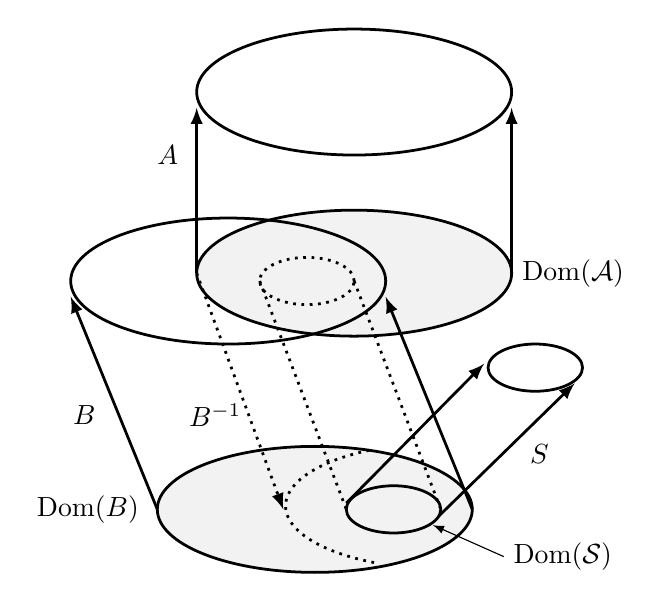
\begin{tikzpicture}
[line width=1pt]
\node at  (1.6+2, 0.1) [right] {$\textrm{Dom}(\seqset{A})$};
\draw[fill=black!5] (1.6, 0.1) ellipse (2cm and 0.8cm); %% Dom A
\draw               (1.6, 2.4) ellipse (2cm and 0.8cm); %% Img A
\draw[-latex] (1.6+2, 0.1)--(1.6+2, 2.4-.2); %% A right
\draw[-latex] (1.6-2, 0.1)--(1.6-2, 2.4-.2); %% A left
\node at  (1.6-2-.1, 1.6) [left] {$A$};
%%
\node at (1.1-2-.1, -2.9) [left] {$\textrm{Dom}(B)$};
\draw[fill=black!5] (1.1, -2.9) ellipse (2cm and 0.8cm); %% Dom B
\draw               (0  ,  0)   ellipse (2cm and 0.8cm); %% Img B
\draw[-latex] (1.1+2, -2.9)--(0+2, 0-.2); %% B right
\draw[-latex] (1.1-2, -2.9)--(0-2, 0-.2); %% B left
\node at  (0.55-2-.1, -1.7) [left] {$B$};
\draw[-latex,dotted] (1.6-2, 0.1)--(0.7, -2.9); %% B-1
\node at (0.3, -1.7) [left] {$B^{-1}$};
\draw[dotted] (1.79, -2.15) arc(118:244: 2cm and 0.8cm); %% Arc
\draw[dotted] (1, 0) ellipse (0.6cm and 0.3cm); %% Dotted S
\draw         (2.1, -2.9) ellipse (0.6cm and 0.3cm); %% Dom S
\draw[dotted] (1-0.6, 0)--(2.1-0.6, -2.9); %% B-1
\draw[dotted] (1+0.6, 0)--(2.1+0.6, -2.9); %% B-1
\draw                     (3.9, -1.1) ellipse (0.6cm and 0.3cm); %% Img S
\draw[-latex] (2.1-0.6, -2.9+.08)    --(3.9-0.6-.05, -1.1+.05); %% Left S
\draw[-latex] (2.1+0.6-.02, -2.9-.08)--(3.9+0.6-.1, -1.1-.2); %% Right S
\node at  (3.7,-2.2) [right] {$S$};
\draw[-latex,thin] (3.5, -3.5) node[right]{$\mathrm{Dom}(\seqset{S})$} -- (2.1+0.5, -2.9-0.2);
\end{tikzpicture}\end{center}

\caption{Proof of \cref{r_invmove}}\label{fig_invmove}
\end{figure}

We see that the set of filesystems the sequences in $\seqset{A}$ do not break intersect with the range of $B$.
As $B$ is a bijection between its domain and range, we can use $B^{-1}$ to map this intersection back
onto the domain of $B$.
As $\worksc{B\cc \seqset{A}}{\seqset{S}}$ the domain of $\seqset{S}$ must be a subset of this
projected intersection.
If so, then we can use $B$ to map the domain of $\seqset{S}$, which yields the domain of $B^{-1}\cc \seqset{S}$.
As it is also a part of the domain of $A$, we get $\worksc{\seqset{A}}{B^{-1}\cc \seqset{S}}$.

The second part of the lemma can be proven in a similar way.
\end{proof}


\begin{mylem}\label{indep_prefix_combine}
The combination of sequences with a common head and independent tails 
continues to work under the same conditions:
\[ \worksc{A\cc B}{\seqset{S}} \wedge \worksc{A\cc C}{\seqset{S}} \wedge B\indep C \Rightarrow \worksc{A\cc B\cc C}{\seqset{S}} \]
\end{mylem}
\begin{proof}
Based on \cref{r_invmove} we know
$\worksc{B}{A^{-1}\cc \seqset{S}}$ and $\worksc{C}{A^{-1}\cc \seqset{S}}$,
and from \cref{combine_independent_sequences} we know
$\worksc{B\cc C}{B,C}$.
Combining these using \cref{workschained}
we get
$\worksc{B\cc C}{A^{-1}\cc \seqset{S}}$. 
Finally, applying the second line of \cref{r_invmove} yields
$\worksc{(A^{-1})^{-1}\cc B\cc C}{\seqset{S}}$, which proves our lemma 
as $\forall\FS: (A^{-1})^{-1}\FS\typeeq A\FS$ (\cref{negneg_is_typeeq}).
\end{proof}



\subsection{The Correctness of Reconciliation}

We are now ready to prove that the proposed algorithm for reconciliation is correct,
that is, applying its result is not going to break the replicas.
We reformulate the original proposition ($\reca\aFS_B\neq\fsbroken$)
based on $\FS_B=B\aFS$, and so we aim to prove that
$B\cc\reca$ is defined wherever $A$ and $B$ are defined:

\begin{myth}\mlabel{reconciliation_correct}
If $A$ and $B$ are simple, then $\worksmbx{A,B}{B\cc \reca}$,
where, to restate \cref{def:reconciliation},
\[ \reca = \ords{\alpha \whr \alpha\in \ambnp  \mbox{~and~}  \alpha\indep \bmanp }. \]
\end{myth}

This is trivial unless $\worksmnilb{A,B}$, so we assume that it is true.
Let us first investigate the part of $A$ and $B$ that is excluded from
$\reca$: their intersection.

\begin{mylem}\mlabel{can_move_intersection}
Let $A$ and $B$ be two simple sequences for which $\worksmnilb{A, B}$.
Then $A$ can be separated into their intersection and the remaining commands:
\[ \acb\cc\amb \in \orderset{A}. \]
\end{mylem}

\begin{proof}
Mark those commands in $A$ that are also in $B$.
We show that
there is an $A'$ in $\orderset{A}$ in which all marked commands are at the beginning.

We show that $A$ can be transformed into $A'$ for which this is true.
We know that if the marked commands are not at the beginning, then
the sequence contains an unmarked command followed by a marked command.
We show that these can be swapped resulting in an equivalent sequence.
Then, by repeating this process similarly to bubble sorting, we arrive at 
a suitable permutation of $A$, which is also equivalent to $A$, and therefore in $\orderset{A}$.

Let us consider therefore the marked command preceded by an unmarked command in $A$,
and let the marked command be $\cxynv$, 
and the preceding unmarked command be $\czwmv$:
\begin{gather*}
A = \cdots\cc  \czwmv\cc  \cxynv\cc  \cdots
\end{gather*}
As $A$ is simple and $\wrks{A}$, from 
\cref{ax_distantrel_breaks,simple_distant_pairs}
we know that these commands can only be on incomparable nodes or form a construction or destruction pair.
In the first case, swapping the commands results in a sequence equivalent to $A$,
and we show that the last two cases are impossible.

In the cases then $\czwmv\cc\cxynv$ is either a construction or a destruction pair,
and, depending on which is the case,
$m=\parent(n)$ or $n=\parent(m)$, respectively.

If $B$ has a command on $m$, let it be $\cqrmv$.
As \cref{simple_distant_pairs} applies to $B$, we know that
$\cxynv$ (which is in $B$), and $\cqrmv$ must also form a construction
or destruction pair.
As $\cxynv$ cannot be both a construction and a destruction command,
this pair must be of the same type as $\czwmv\cc\cxynv$,
and as the relationship between $n$ and $m$ is given,
we know $\cqrmv$ must precede $\cxynv$ in $B$.

Because the output value of the first command in construction
and destruction pairs is determined by the type of the pair,
$r=w$.
Also, as $\worksmnilb{A,B}$, 
from \cref{worksinputmatch}
we know that $[q]=[z]$.
Therefore $\cqrmv=\czwmv$,
which is a contradiction as $\czwmv$ was not marked,
but we see it must also be in $B$.

The last remaining case is when there is no command on $m$ in $B$.
Let $B'$ be $B$
with an extra assertion command added just before $\cxynv$
according to \cref{ax_child_assert,ax_parent_assert}, 
from which we know that $B'\equiv B$.
Let the new command be $\cqrmv$.
As $B'$ is still minimal (but no longer simple),
the argument above applies, and we again know
that $[q]=[z]$ and $r=w$.
As $\cqrmv$ is an assertion command, $[q]=[r]$ also holds,
from which $[z]=[w]$ (as $[z]=[q]=[r]=[w]$), which is a contradiction
as $A$ contains no assertion commands.
\end{proof}

We would like to prove that $\worksmbx{A,B}{B\cc \reca}$.
From \cref{can_move_intersection} above we know that we can move commands in $\acbnp$
to the beginning of $A$ and $B$, and so this is equivalent to
\[ \worksm{\big\{\acb\cc\amb,~ \acb\cc\bma\big\}}{\acb\cc \bma\cc \reca}. \]

For ease of reading, let us rename
\begin{itemize}
\item $\amb$ to $S$,
\item $\reca$ to $S^*$,
\item $\bma$ to $T$,
\item and $\acb$ to $U$.
\end{itemize}
In this notation, we intend to prove that
\[ \worksmbx{U\cc S,U\cc T}{U\cc T\cc S^*}. \]
We can do so if we can show that
\[ \worksmbx{S,T}{S^*}. \]

This is because from $\worksmbx{S,T}{S^*}$ trivially $\worksmbb{S,T}{S^*, T}$,
and from $S^* \indep T$ and \cref{combine_independent_sequences} we know 
$\worksmbx{S^*,T}{T\cc S^*}$.
Combining the two we get $\worksmbx{S,T}{T\cc S^*}$,
which using \cref{works_restricted} yields
$\worksm{U\cc\{S,T\}}{U\cc T\cc S^*}$, that is,
$\worksmbx{U\cc S,U\cc T}{U\cc T\cc S^*}$.

To restate some results above, we therefore already know the following:
\begin{itemize}
\item $S=\amb$ and $T=\bma$ are simple as $A$ and $B$ are simple
\item $S\cap T = \amb \cap \bma = \emptyset$
\item $S^*$ is the largest subset of $S$ for which $S^*\indep T$, as
$\reca$ is the largest subset of $\amb$ for which $\reca\indep\bma$.
\end{itemize}
Our theorem is therefore proven if we prove the following lemma.
\newcommand{\condSimple}{(c1)}
\newcommand{\condDisj}{(c2)}
\newcommand{\condApr}{(c3)}
\begin{mylem}\mlabel{reconciliation_correct_part}
If
{\rm\condSimple} $S$ and $T$ are simple sequences,
{\rm\condDisj} $S\cap T=\emptyset$,
and {\rm\condApr} $S^*$ is the largest subset of $S$ where $S^*\indep T$,
then
$\worksmbx{S,T}{S^*}$.
\end{mylem}
\begin{proof}
This is trivial unless $\worksmnilb{S,T}$, so we assume that it is the case.
The proof is similar to that of \cref{can_move_intersection}.
We mark all commands in $S$ that are in its subset $S^*$, and
we prove that $S$ can be transformed into $S'$
where all marked commands are at the beginning.
If so, then 
$\worksm{S}{S^*}$ based on \cref{worksextpostfix},
from which we get $\worksmbx{S,T}{S^*}$.

Again we know that if $S$ does not already have all marked commands at its beginning,
then there is an unmarked command followed by a marked one.
We show that these commands are independent and so they can be swapped
resulting in an equivalent sequence.
By repeating this process we can generate a suitable $S'$.

Let therefore the marked command in $S$ be $\cxynv$
and the preceding unmarked command be $\czwmv$.
As $S$ is simple and $\wrks{S}$, from 
\cref{ax_distantrel_breaks,simple_distant_pairs}
we know that these commands can only be on incomparable nodes or form a construction or destruction pair.
In the first case, swapping the commands results in a sequence equivalent to $S$,
and we show that the other two cases are not possible as they would lead to contradiction.

In the last two cases, we know that either $m=\parent(n)$ or $n=\parent(m)$.
We also know that because of {\condApr} there must be 
a command $\cqrov$ in $T$ which is not independent of $\czwmv$
as $\czwmv$ is not part of $S^*$.
% \begin{gather*}
% S = \cdots\cc  \czwmv\cc  \cxynv\cc  \cdots \\
% T = \cdots\cc  \cqrov\cc \cdots
% \end{gather*}
Based on \cref{incomparable_is_independent} we know this means that
either $m\descendantEq o$ or $o\descendantEq m$.
From {\condApr} we also know that $\cxynv\indep \cqrov$,
and so because of \cref{incomparable_is_independent},
$n\unrel o$.
We also know none of these commands is an assertion command, and 
from {\condDisj} that $\cqrov\neq\czwmv$.

We therefore have four cases considering the relationships between $n,m$ and $o$:
\begin{itemize}
\item $n=\parent(m)$ and $o\descendantEq m$.
   This would mean that $o\descendantEq n$ or $n=\parent(o)$ (if $o=m$), which contradicts $n\unrel o$.
\item $n=\parent(m)$ and $m\descendantEq o$.
   This would mean that $n\descendant o$, which contradicts $n\unrel o$.
\item $m=\parent(n)$ and $o\descendantEq m$.
   This would mean that $o\descendant n$, which contradicts $n\unrel o$.
\item $m=\parent(n)$ and $m\descendantEq o$.
   Let us continue with this case.
\end{itemize}

As $m=\parent(n)$, we know $\czwmv\cc\cxynv$ must be a construction pair.
We know that $T$ cannot have a command on $m$ as $m=\parent(n)$ and $\cxynv\indep T$,
and so $m\neq o$ and therefore $m\descendant o$.
This means we can create a new sequence $T'\equiv T$ by inserting a command on 
$m$ into $T$ before $\cqrov$
according to \cref{ax_parent_assert}, the input type of which is $[\vald]$.
As $T'$ is still minimal, and $\worksmnilb{S,T}$,
from \cref{worksinputmatch} we get $[z]=[\vald]$, which is a contradiction,
as $\czwmv$ is the first command in a construction pair.
\end{proof}



\subsection{Reconciliation is Maximal}

% Reconciliation is maximal
% -------------------------
% This is where we're using |D|=1

%% TODO general properties of commands ==> behavior on specific filesystems

The reconciliation algorithm defined above is also maximal, that is,
it is not possible to apply any further commands from $A\setminus B$ to $\FS_B$.
To show this, we are going to prove the following theorem:

\begin{myth}\label{rec_is_complete}
If $A$ and $B$ are simple sequences,
and we select a sequence $S\subset \amb$ so that
it contains a command $\cxynv$ for which $\cxynv\nindep\bma$,
then $B\cc S$ either breaks all filesystems $A$ and $B$ do not break
(that is, $S$ breaks all possible $\FS_B$ replicas),
or it changes a node that $B$ has already changed to a different value,
that is, it overrides a change in $\FS_B$.
\end{myth}
Such an override could occur if a given node was modified differently in
$A$ and $B$ (to different values but the same type), which is clearly
a conflict that should be marked for review
by a human or a different system.
\begin{proof}
The proof is similar to the ones we have seen above.
Without loss of generality, we assume that $\cxynv$ is the first command in $S$
that is not independent of $\bmanp$.
If so, we can split $S$ into $S_0\cc\cxynv\cc S_1$ where $S_0\indep\bma$.
Let us also split $\bmanp$ into $T_0\cc\czwmv\cc T_1$ where $T_1\indep\cxynv$.
From \cref{can_move_intersection} we know that
$B\cc S \equiv \acb\cc\bma\cc S$.
We also know that commands in $S_0$ and $\bmanp$ commute, and so this is equivalent to
$\acb\cc S_0\cc\bma\cc\cxynv\cc S_1$.
Expanding $\bmanp$ and swapping $T_1$ and $\cxynv$ we get
\[ \acb\cc S_0\cc T_0 \cc \czwmv \cc \cxynv\cc T_1\cc S_1. \]

First, we prove that this sequence breaks all filesystems
unless $n=m$.
Let us therefore suppose $n\neq m$ and, to use an inverse proof,
that the sequence is defined on $\FS$ where $A\aFS\neq\fsbroken$.
If so, its initial segment, $\acb\cc S_0\cc T_0 \cc \czwmv \cc \cxynv$ must also be defined.

We know $\cxynv\nindep\czwmv$, and so from \cref{incomparable_is_independent}, $n\nunrel m$.
As the sequence is defined, $\czwmv\cc\cxynv$ can only be a construction or destruction pair.
As $\czwmv$ and $T_0$ originate from $\bmanp$ and $B$ is simple, we also know there are
no commands on $m$ in $\acbnp$ or $T_0$,
and that there are no commands on $m$ in $S_0$ as $S_0\indep\bma$.

On the one hand we therefore know that $\FS(m)$ must be of type $[z]$,
but on the other, from \cref{ax_directchild_breaks,ax_directparent_breaks},
we also know that $\cxynv$ cannot be applied to $\FS$ without
changing $\FS(m)$ first.
As $A\aFS\neq\fsbroken$, this means that $A$ must contain a command on $m$.
Let this command be $\cqrmv$.

Clearly $[q]=[z]$ (from \cref{worksinputmatch}), and from the construction and destruction
pairs we also see that $r=w$ must hold, where $w=\vald$ or $w=\empt$.
As $|\setd|=1$ and $|\setb|=1$, this also means that $::v_R=v_W::$ and therefore
$\cqrmv = \czwmv$.
This is a contradiction as $\cqrmv\in A$, but $\czwmv\in\bmanp$.

The only possibility is therefore $n=m$.
As $A$ and $B$ are simple, we therefore know that these are the first commands on $n$,
and so (again from \cref{worksinputmatch}) $[z]=[x]$.
We also know $w\neq y$ as otherwise the two commands would be equal and
would be included in $\acbnp$,
but this means that $\cxynv$, from $A$, overrides a change introduced 
by $\czwnv$, from $B$, which should be treated as a conflict.
\end{proof}

From the proof it is apparent that this result depends on $|\setd|=1$.



% section

\section{Related Work}\mlabel{sec_relatedwork}

\subsection{Liberal and Conservative Reconciliation}

We consider the reconciliation algorithm described here an improvement over
the one derived during our previous research \cite{NREC}
as the previous algorithm not only fails to propagate all possible commands
wherever it is possible (that is, where it does not break the filesystem),
but the current algorithm is also simpler.
This is because the previous reconciliation algorithm excludes
commands from being propagated which must be preceded by a command that conflicts.

The former observation is supported by Berzan and Ramsey, who in \cite{CBNR} 
describe different general reconciliation policies.
The liberal (maximal) policy propagates all updates to all replicas where
the update does not break the filesystem, while a conservative policy
refrains from updating any node that is below a node with conflicting commands.
They show that the reconciliation algorithm in \cite{NREC} implements
an intermediate policy as one can easily construct two- or three-replica scenarios
where an update could clearly be propagated, but it is excluded.
To rephrase the example in \cite{CBNR}, consider the following two
update sequences that have been applied to replicas $\FS_A$ and $\FS_B$:
\begin{align*}
A&=\caaa{\empt}{\valdi}{\pn}\cc\caaa{\empt}{\valf}{n} \\
B&=\caaa{\empt}{\valdii}{\pn}
\end{align*}
(\cite{NREC} did not require all directories to have the same value).
Clearly $\caaa{\empt}{\valf}{n}$ could be applied to $\FS_B$, but it is not as
it must be preceded by creating the directory, which conflicts with the same command in $B$
due to the different value.
(Introducing a third replica which has not changed at all further complicates the picture.)
The current algorithm no longer needs to specify that there can be no conflicts
on preceding commands, and, to use the above terminology, implements a fully liberal policy.


\subsection{Comparing Definitions of Conflicts}

As a test of the proposed reconciliation algorithm, 
we compare our definition of conflicting
updates to how conflicts are defined by Balasubramaniam and Pierce
in their state-based approach implemented in the Unison synchronizer \cite{BP}.
As we noted in \cite{NREC}, the update detector they describe provides a safe estimate of nodes
(paths) at which updates occurred.
It marks some nodes as \emph{dirty} in a way that we know that at non-dirty nodes
the filesystems (replicas) have not changed between their common original state and current state
(see Definition 3.1.1 in \cite{BP}).
The \emph{dirty} marks are also up-closed, that is, all ancestor nodes of a dirty node
are also dirty (Fact 3.1.3 in \cite{BP}).
And finally, in our notation, 
a conflict is detected between replicas $\FS_A$ and $\FS_B$ at node $n$
if $n$ is marked as dirty in both $\FS_A$ and $\FS_B$, and
$\FS_A(n)\neq\FS_B(n)$, and $n$ does not point to a directory in both replicas.
(In other words, 
$[\FS_A(n)]\neq[\vald]$ or $[\FS_B(n)]\neq[\vald]$; see section 4.1 in \cite{BP}.
Let us note that there is an alternative approach to defining an algorithm for
the same synchronizer by Pierce and Vouillon in \cite{PV}.)

It can be easily seen that due to an edge case, 
not all conflicts detected based on the above definition
entails a conflict based on our system; that is, \cite{BP} describes a more
conservative policy.
We use the example we described in \cite{NREC},
where $\FS(\pn)$ is a directory and $\FS(n)$ is a file, and
the two replicas are derived in the following way:
\begin{gather*}
\FS_A = (\cfba{n} \cc \cdba{\pn}) \aFS \\
\FS_B = \cfba{n} \aFS.
\end{gather*}
Then, $\pn$ is dirty in both replicas:
in $\FS_A$ it was modified, and in $\FS_B$ one of its descendants was modified.
Moreover, $\FS_A(\pn)\neq\FS_B(\pn)$ and $[\FS_A(\pn)]\neq[\vald]$ as it is empty.
Therefore, a conflict is detected at $\pn$.
(This behavior is preserved in the more recent Harmony synchronizer.
See ``delete/delete conflicts'' in \cite{PSG,FGKPS}.)
Our reconciliation algorithm detects no conflicts;
instead, it propagates $\cdba{\pn}$ to $\FS_B$, which we think is as expected
and desired.

At the same time, it can be shown that if our command-based reconciler
detects a conflict, it entails a conflict in the state-based reconciler.
We note here that Balasubramaniam and Pierce also suppose that all directories are equal,
therefore, as elsewhere, we are safe to continue to assume that $|\setd|=1$.

\begin{proof}
Let $A$ and $B$ be two simple sequences returned by the update detector
for the two replicas $\FS_A$ and $\FS_B$.
A conflict between the commands $\cxynv\in A$ and $\czwmv\in B$
means that even though $\cxynv\in A\setminus B$
and $\czwmv\in B\setminus A$, they cannot be included in
$\reca$ and $\recb$, respectively, because
$\cxynv\nindep\czwmv$ (see \cref{def:reconciliation}).

From \cref{incomparable_is_independent} we therefore know that $n\nunrel m$.
Without loss of generality we can assume that $n\descendantEq m$.
From this we see that $n$ is \emph{dirty} in both $\FS_A$ and $\FS_B$,
as the filesystem changes at $n$ in $\FS_A$ and at $n$ or its descendant in $\FS_B$
(and none of the commands are assertion commands).

Now we only need to show that $\FS_A(n)\neq\FS_B(n)$, because from this 
and $|\setd|=1$ we will also
know that at least one of these values is not a directory,
and therefore there is a conflict at $n$ in the state-based reconciler.

If $n=m$, this follows from the fact that $\cxynv\neq\czwmv$ 
(because they are not in $A\cap B$),
as from \cref{worksinputmatch} we have $[x]=[z]$,
and therefore necessarily $y\neq w$,
that is, $\FS_A(n)=y\neq w=\FS_B(n)$.

If $n\descendant m$ and there is no command on $n$ in $B$, then 
because $\cxynv$ is not an assertion command, we again have
$\FS_A(n)\neq\FS(n)=\FS_B(n)$, where $\FS$ is the common ancestor of the replicas.
Finally, if there is a command on $n$ in $B$, then 
from $\cxynv\in A\setminus B$ we know
it must be different from $\cxynv$, and similarly to the first case,
we have $\FS_A(n)\neq\FS_B(n)$.
\end{proof}



% section

\section{Towards a Filesystem-Free Algebra}\mlabel{sec_algebra}

Similarly to \cite{NREC} we can consider creating an algebra over command sequences
which would enable us to draw conclusions about the behaviors of the sequences
without considering the underlying filesystems.
This would provide a secondary model of (filesystem) commands above (and independent of) the model of filesystems
defined in this paper. The new model would no longer describe filesystems as such,
but would use known relationships between sequences of commands as its starting point.

In this algebra, equivalence ($\equiv$) and extension ($\eqext$) would become algebraic relations
between sequences, and logical rules involving them
(e.g. $ A\equiv B \Rightarrow S\cc A\cc T\equiv S\cc B\cc T $) would be re-cast as inference rules.
In addition to these, the \namecrefs{ax_separate_commute} listed in \cref{section_axioms}
would become axioms that we accept as true, and from which other true statements can be derived
using the inference rules.
Such a system would allow us to deduce, for example, whether two sequences are equivalent
or one extends the other without reference to filesystems.

We note, however, that the \namecrefs{ax_separate_commute} to be used as axioms 
specify the relationships between the nodes
the commands act on, which would require a more complicated set of symbols to represent
in the new algebra.
To avoid this, we think it will be more fruitful to regard commands (and sequences)
on different nodes as different, and, in effect, have nine times as many commands 
in the algebra as there are nodes in the namespace of the filesystems.
This will allow us to reduce the number of types of symbols in our algebra, and regard
the \namecrefs{ax_separate_commute} not as axioms, but as templates for axioms
from which all axioms (for pairs of separate nodes, etc.) can be generated.

We expect that the soundness and completeness of such an algebra can be proven
similarly to the proofs described in \cite{NREC}.
Indeed, results in the current paper can serve as building blocks of such a proof:
derivations in \cref{axiom_proof} for the \namecrefs{ax_separate_commute}
in effect proves the soundness of all axioms,
and \cref{simple_reorder_equiv} proves completeness in a limited sense.
It is also worth noting that the majority of proofs presented in this paper
do not actually refer to specific filesystems or the definition of commands,
but draw on known relationships between the commands themselves.
In other words, many proofs are transferable to the algebra that we describe here.

In a more complete algebra from which the correctness and completeness
of reconciliation could also be derived,
one would also include symbols, inference rules and axioms for 
$\worksmnil{\seqset{A}}$ and $\worksm{\seqset{A}}{\seqset{B}}$.
We see proving the soundness and completeness of this extended algebra
an intriguing problem that is worthy of further research.


% section

\section{Conclusions and Further Research}

Apart from constructing an algebra,
there are many other ways in which further work can extend the current results.
An important extension would be to
consider reconciling not only two, but more replicas in a single step and
prove the correctness and maximality of the algorithm proposed,
or show that it is impossible to satisfy these criteria.

A related problem is to extend the system and the proofs
to allow for cases where reconciliation cannot
complete fully
or if only a subset of the replicas are reconciled 
(e.g. due to network partitioning),
both of which would result in a state where different replicas
have different common ancestors, that is,
the updates specific to the replicas start from different points
in the update history of the filesystem.
Existing research can offer pointers as to how such cases can be modelled
in our algebraic system.
Parker et al. \cite{PPRS} and Cox and Josephson \cite{CJ}
describe version vectors (update histories) kept as metadata,
while Chong and Hamadi present distributed algorithms that allow incremental synchronization \cite{CH}.
Representing individual updates to files
in their modification histories (as described in \cite{CJ})
as separate commands could also enable an algebraic synchronizer to reconcile otherwise
conflicting updates and resolve partial reconciliations.

An extension of our results could also entail relaxing
the simplifying assumptions we used.
Identifying which results depend on the assumption that $|\setd|=1$
and devising updated proofs and algorithms for when $|\setd|>1$,
or specifying a pre-processing step that reconciles meta-information in directories
can enable the synchronizer
to identify and resolve a wider range of conflicts.
Similarly, designing pre- and post-processors that
present removing and creating a node
not as separate updates but as a single rename (move),
could contribute to the user-friendliness of the reconciler
and help avoid human error.

And finally, we hope that this work, together with \cite{NREC}, provides
a blueprint of constructing an algebra of commands for different storage protocols
(e.g. XML trees, mailbox folders, generic relational databases, etc.),
and of demonstrating the adequacy and completeness of update and conflict detection and reconciliation
algorithms defined over it.
This, in turn, can offer formal verification of the algorithms underlying
specific implementations in a variety of synchronizers.
Alternatively, by generalizing the parent--child relationships between filesystem nodes,
the demonstrated properties of minimal sequences of commands
and conditional operation of sequences ($\workssign$)
may also contribute to future research into algebraic structures
constrained by predefined sparse connections between their elements.


\section{Acknowledgments}

% TODO Add reviewer
% TODO Consider below
I thank L. Csirmaz for his invaluable input on this paper,
and Bill Zissimopoulos for his observations on algebraic file synchronization that triggered this research.

\begin{thebibliography}{99}


% B 4
\bibitem{BP}
S. Balasubramaniam and Benjamin C. Pierce,
``What is a File Synchronizer?''
in \emph{Proceedings of the 4\textsuperscript{th} Annual 
ACM/IEEE International Conference on Mobile Computing and Networking,}
New York: ACM, 1998, pp. 98--108.

% B 21
\bibitem{CBNR} 
Constantin Berzan and Norman Ramsey,
``Summer Scholars Technical Report,''
Medford, MA: Tufts University, 2010.
Accessed 29 November 2015.
http://thirld.com/files/summerscholars\_techreport.pdf.

% C 8
\bibitem{CJ}
Russ Cox and William Josephson,
``File synchronization with Vector Time Pairs,''
MIT CSAIL Technical Report,
Cambridge, MA: MIT,
2005.
Accessed 22 November 2015.
http://hdl.handle.net/1721.1/30527.

% K 3
\bibitem{KRSD}
Anne-Marie Kermarrec and Antony Rowstron and Marc Shapiro and Peter Druschel,
``The IceCube Approach to the Reconciliation of Divergent Replicas,''
in \emph{Proceedings of the Twentieth Annual ACM Symposium on Principles of Distributed Computing,}
New York: ACM, 2001, pp. 210--218.

% P 6
\bibitem{PPRS}
% Parker, D. S. and Popek, G. J. and Rudisin, G. and Stoughton, A. and Walker, B. J. and Walton, E. and Chow, J. M. and Edwards, D. and Kiser, S. and Kline, C.
D. S. Parker et al.,
``Detection of Mutual Inconsistency in Distributed Systems,''
in \emph{IEEE Trans. Softw. Eng.,}
vol. 9, no. 3,
Piscataway, NJ: IEEE Press,
May 1983,
pp. 240--247.

% P 14
\bibitem{PV}
Benjamin C Pierce and J{\'e}r{\^o}me Vouillon,
``What's in Unison? A formal specification and reference implementation of a file synchronizer,''
\emph{Technical Reports (CIS),}
Paper 40,
Philadelphia, PA: U of Pennsylvania,
2004.
Accessed 23 November 2015.
http://repository.upenn.edu/cis\texttt{\detokenize{_}}reports/40.

% R
\bibitem{NREC} 
Norman Ramsey and Elod Csirmaz,
``An Algebraic Approach to File Synchronization,''
in \emph{Proceedings of the Joint 8\textsuperscript{th} European Software Engineering Conference 
and 9\textsuperscript{th} ACM SIGSOFT Symposium on the Foundations of Software Engineering,}
New York: ACM, 2001, pp. 175--185.

% T 1
\bibitem{TSR}
Vinh Tao and Marc Shapiro and Vianney Rancurel,
``Merging Semantics for Conflict Updates in Geo-distributed File Systems,''
in \emph{Proceedings of the 8\textsuperscript{th}
 ACM International Systems and Storage Conference,}
New York: ACM, 2015, pp. 10:1--10:12.

% T 5
\bibitem{TTPDSH}
% D. B. Terry and M. M. Theimer and Karin Petersen and A. J. Demers and M. J. Spreitzer and C. H. Hauser
D. B. Terry et al.,
``Managing Update Conflicts in Bayou, a Weakly Connected Replicated Storage System,''
in \emph{Proceedings of the Fifteenth ACM Symposium on Operating Systems Principles,}
New York, NY: ACM, 1995, pp. 172--182.

% Z
\bibitem{BZ}
Bill Zissimopoulos, personal communication, August 2015.


\end{thebibliography}

\appendix

\section{Proofs for Rules}\mlabel{axiom_proof}

In this section we offer proofs for the \namecrefs{ax_separate_commute} listed in
\cref{rules_lemma}.
For the purposes of the proofs we extend the notion of filesystems 
to the full set of functions mapping $\setn$ to $\setv$, even if they
do not have the tree property.
In this case we continue to say that the filsystem is broken,
but we also describe the filesystem values at certain nodes.
Also, in order to pinpoint the region that violates the tree property,
we say that the filesystem is \emph{broken at $n$} if 
$n$ is not a dictionary, but has at least one non-empty child.

Accordingly, we also extend filsystem commands from partial to full functions,
and assume that they return a filesystem we can describe in all cases.
We note that once a filesystem is broken, it stays broken, even if
after a subsequent command it no longer violates the tree property.

It follows from the definition of the tree property that
whether a filesystem is \emph{broken at a node $n$} is determined only
by the values at $n$, $\parentf{n}$, and the children of $n$.
In other words,

\begin{myclm}[Locality of tree property violations]\mlabel{broken_local}
If two filesystems over $\setn$ have the same values at a node $n$,
$\parentf{n}$ (if exists), and at all children of $n$ (if they exist),
then either both filesystems are broken at $n$, or none of them are.
\end{myclm}

\cref{ax_separate_commute}

We use an inverse proof and assume $\cxynv\cc\czwmv \nequiv \czwmv\cc\cxynv$.
Since the values in the resulting filesystems are the same,
this is only possible if, for an initial non-broken filesystem $\FS$,
one side results in a broken filesystem, and the other side does not.
Without loss of generality, we can assume
$(\cxynv\cc\czwmv)\aFS$ is not broken, but $(\czwmv\cc\cxynv)\aFS$ is.
This means that either $\czwmv\aFS$ is already broken, or it is not, and applying $\cxynv$
breaks the filesystem.

In the former case, the filesystem must be broken at $m$ or $\parentf{m}$.
Since the set of $n$ with its granparent, parent and children; and $m$ with its grandparent, parent and children
are disjunct, we know $\cxynv\aFS$ contains the same values around $m$ as $\aFS$.
This leads to contradiction as from \cref{broken_local} we know
that being broken at $m$ or $\parentf{m}$
... WHAT ABOUT SIBLINGS? ...
while applying $\czwmv$ to $\cxynv\aFS$ on the left-hand side resulted in a working filesystem,
it resulted in a broken filesystem when applied to $\FS$ on the right-hand side.
The proof is similar in the case when applying $\cxynv$ breaks the filesystem on the right-hand side.


\end{document}
